\documentclass[12pt, titlepage]{article}

\usepackage{amsmath, mathtools}

\usepackage[round]{natbib}
\usepackage{amsfonts}
\usepackage{amssymb}
\usepackage{graphicx}
\usepackage{colortbl}
\usepackage{xr}
\usepackage{hyperref}
\usepackage{longtable}
\usepackage{xfrac}
\usepackage{tabularx}
\usepackage{float}
\usepackage{siunitx}
\usepackage{booktabs}
\usepackage{multirow}
\usepackage[section]{placeins}
\usepackage{caption}
\usepackage{fullpage}
\usepackage{amsfonts}

\hypersetup{
bookmarks=true,     % show bookmarks bar?
colorlinks=true,       % false: boxed links; true: colored links
linkcolor=red,          % color of internal links (change box color with linkbordercolor)
citecolor=blue,      % color of links to bibliography
filecolor=magenta,  % color of file links
urlcolor=cyan          % color of external links
}

\usepackage{array}

\externaldocument{../../SRS/SRS}

%% Comments

\usepackage{color}

\newif\ifcomments\commentstrue %displays comments
%\newif\ifcomments\commentsfalse %so that comments do not display

\ifcomments
\newcommand{\authornote}[3]{\textcolor{#1}{[#3 ---#2]}}
\newcommand{\todo}[1]{\textcolor{red}{[TODO: #1]}}
\else
\newcommand{\authornote}[3]{}
\newcommand{\todo}[1]{}
\fi

\newcommand{\wss}[1]{\authornote{blue}{SS}{#1}} 
\newcommand{\plt}[1]{\authornote{magenta}{TPLT}{#1}} %For explanation of the template
\newcommand{\an}[1]{\authornote{cyan}{Author}{#1}}

%% Common Parts

\newcommand{\progname}{Software Engineering} % PUT YOUR PROGRAM NAME HERE
\newcommand{\authname}{Team \#11, OKKM Insights
\\ Mathew Petronilho
\\ Oleg Glotov
\\ Kyle McMaster
\\ Kartik Chaudhari} % AUTHOR NAMES                  

\usepackage{hyperref}
    \hypersetup{colorlinks=true, linkcolor=blue, citecolor=blue, filecolor=blue,
                urlcolor=blue, unicode=false}
    \urlstyle{same}
                                


\begin{document}

\title{Module Interface Specification for \progname{}}

\author{\authname}

\date{\today}

\maketitle

\pagenumbering{roman}

\section{Revision History}

\begin{tabularx}{\textwidth}{p{3cm}p{2cm}X}
\toprule {\bf Date} & {\bf Version} & {\bf Notes}\\
\midrule
Date January 17th & 1.0 & \\
\bottomrule
\end{tabularx}

~\newpage

\section{Symbols, Abbreviations and Acronyms}

See SRS Documentation \href{https://github.com/OKKM-insights/OKKM.insights/tree/main/docs/SRS}{here}

\newpage

\tableofcontents

\newpage

\pagenumbering{arabic}

\section{Introduction}

The following document details the Module Interface Specifications for
OrbitWatch, a crowdsourced datalabelling platform which aims to improve the process of extracting information from satelite images.

Complementary documents include the System Requirement Specifications
and Module Guide.  The full documentation and implementation can be
found at \url{https://github.com/OKKM-insights/OKKM.insights/}

\section{Notation}

% \wss{You should describe your notation.  You can use what is below as
%   a starting point.}

The structure of the MIS for modules comes from \citet{HoffmanAndStrooper1995},
with the addition that template modules have been adapted from
\cite{GhezziEtAl2003}.  The mathematical notation comes from Chapter 3 of
\citet{HoffmanAndStrooper1995}.  For instance, the symbol := is used for a
multiple assignment statement and conditional rules follow the form $(c_1
\Rightarrow r_1 | c_2 \Rightarrow r_2 | ... | c_n \Rightarrow r_n )$.

The following table summarizes the primitive data types used by \progname. 

\begin{center}
\renewcommand{\arraystretch}{1.2}
\noindent 
\begin{tabular}{l l p{7.5cm}} 
\toprule 
\textbf{Data Type} & \textbf{Notation} & \textbf{Description}\\ 
\midrule
character & char & a single symbol or digit\\
integer & $\mathbb{Z}$ & a number without a fractional component in (-$\infty$, $\infty$) \\
natural number & $\mathbb{N}$ & a number without a fractional component in [1, $\infty$) \\
real & $\mathbb{R}$ & any number in (-$\infty$, $\infty$)\\
date & Date & provides a specific date and time\\
\bottomrule
\end{tabular} 
\end{center}

\noindent
The specification of \progname \ uses some derived data types: sequences, strings, and
tuples. Sequences are lists filled with elements of the same data type. Strings
are sequences of characters. Tuples contain a list of values, potentially of
different types. In addition, \progname \ uses functions, which
are defined by the data types of their inputs and outputs. Local functions are
described by giving their type signature followed by their specification.

\section*{System Components}

\subsection*{MLModel}
Represents a machine learning model, identified by attributes such as:
\begin{itemize}
    \item \textbf{model\_name}
    \item \textbf{model\_path}
    \item \textbf{model\_type}
    \item Metadata about the model (e.g., training parameters, architecture)
\end{itemize}

\subsection*{ModelTrainingRun}
Captures the details of a model's training process, including:
\begin{itemize}
    \item \textbf{training\_data\_path}
    \item Evaluation metrics
    \item Parameters used during training
\end{itemize}

\subsection*{ModelEvaluationRun}
Represents the evaluation process for a model, containing:
\begin{itemize}
    \item \textbf{evaluation\_data\_path}
    \item Evaluation metrics (e.g., precision, recall)
\end{itemize}

\subsection*{ModelDeployment}
Tracks the deployment details of a machine learning model, such as:
\begin{itemize}
    \item \textbf{deployment\_environment} (e.g., Production, Staging)
    \item \textbf{deployment\_date}
\end{itemize}

\subsection*{Account}
Describes user accounts in the system with attributes like:
\begin{itemize}
    \item \textbf{username}
    \item \textbf{email}
    \item \textbf{account\_type} (e.g., Client, Labeler, Admin)
    \item Security-related fields such as \textbf{password\_hash} and \textbf{last\_login}
\end{itemize}

\subsection*{AccountModification}
Maintains a log of changes made to user accounts, tracking:
\begin{itemize}
    \item \textbf{field\_modified}
    \item \textbf{old\_value}
    \item \textbf{new\_value}
\end{itemize}

\subsection*{LoginAttempt}
Records login attempts for security purposes, including:
\begin{itemize}
    \item \textbf{username}
    \item \textbf{attempt\_time}
    \item Whether the attempt was successful
\end{itemize}

\subsection*{Project}
Defines a labeling or analysis project, identified by:
\begin{itemize}
    \item \textbf{project\_name}
    \item \textbf{description}
    \item Associated metadata
\end{itemize}

\subsection*{User}
Represents individuals (e.g., labelers, managers) working within the system, including:
\begin{itemize}
    \item \textbf{username}
    \item \textbf{role}
\end{itemize}

\subsection*{ProjectAssignment}
Tracks which users are assigned to specific projects, identified by:
\begin{itemize}
    \item \textbf{project\_id}
    \item \textbf{user\_id}
\end{itemize}

\subsection*{SatelliteImage}
Represents images (e.g., satellite imagery) linked to specific projects, with attributes like:
\begin{itemize}
    \item \textbf{image\_path}
    \item \textbf{acquisition\_date}
\end{itemize}

\subsection*{LabelingTask}
Encapsulates a labeling activity, defined by:
\begin{itemize}
    \item \textbf{status}
    \item \textbf{start\_time}
    \item \textbf{end\_time}
    \item The user assigned to the task
\end{itemize}

\subsection*{Report}
Represents generated reports for projects, with fields like:
\begin{itemize}
    \item \textbf{report\_data}
    \item \textbf{generation\_date}
    \item The user who generated the report
\end{itemize}

\subsection*{ServiceRequest}
Tracks requests for services such as image acquisition or data processing, with attributes like:
\begin{itemize}
    \item \textbf{request\_type}
    \item \textbf{status}
\end{itemize}

\subsection*{Image}
Represents standalone images within the system, identified by:
\begin{itemize}
    \item \textbf{image\_path}
    \item \textbf{upload\_date}
\end{itemize}

\subsection*{Labeller}
Represents individuals performing labeling tasks, identified by:
\begin{itemize}
    \item \textbf{labeller\_name}
\end{itemize}

\subsection*{Object}
Represents specific objects detected in an image, with attributes like:
\begin{itemize}
    \item \textbf{bounding\_box\_coordinates}
    \item \textbf{object\_type}
\end{itemize}

\subsection*{Label}
Represents annotations made by a labeller, linking to specific objects in an image and storing information like:
\begin{itemize}
    \item \textbf{label\_text}
    \item \textbf{timestamp}
    \item \textbf{labeller\_id}
\end{itemize}

The following diagram display additional details on the relationship between datatypes\\ 
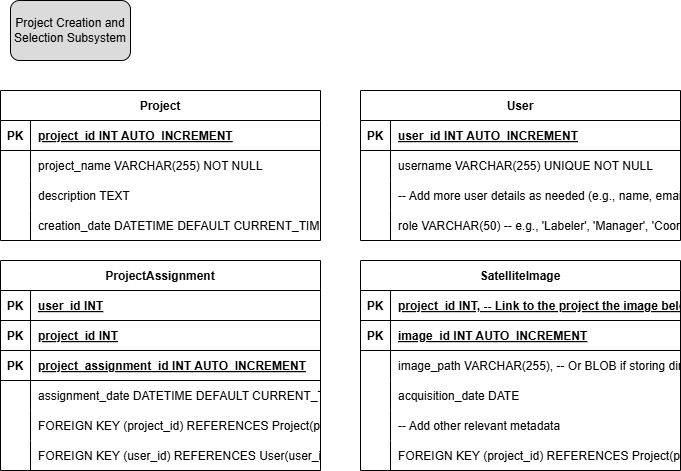
\includegraphics[scale=0.5]{dt3.png}\\
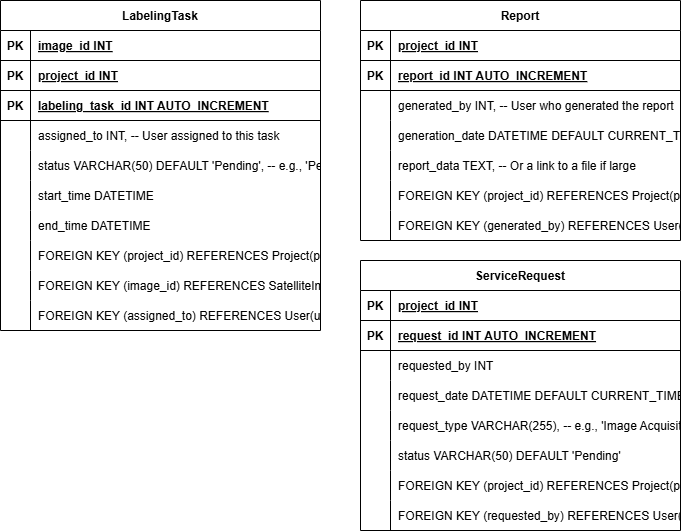
\includegraphics[scale=0.5]{dt4.png}\\
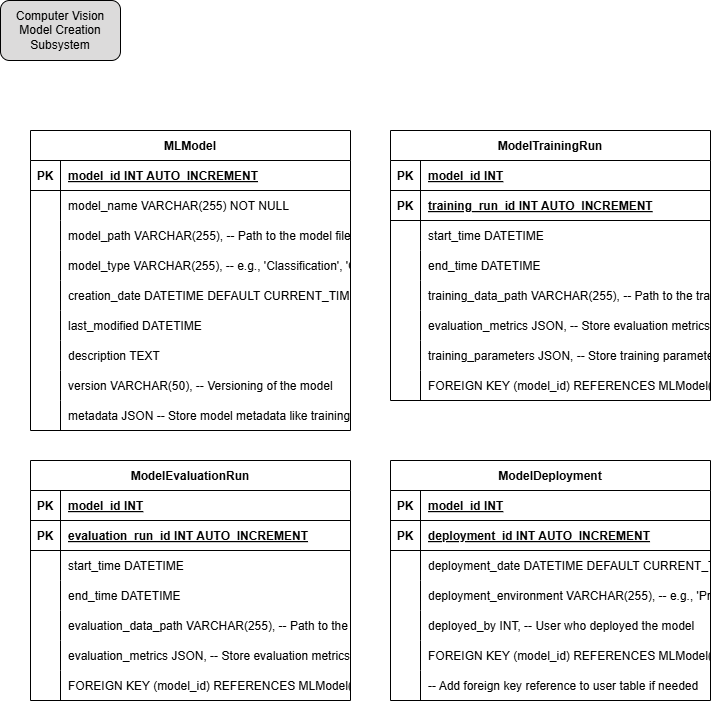
\includegraphics[scale=0.5]{dt1.png}\\
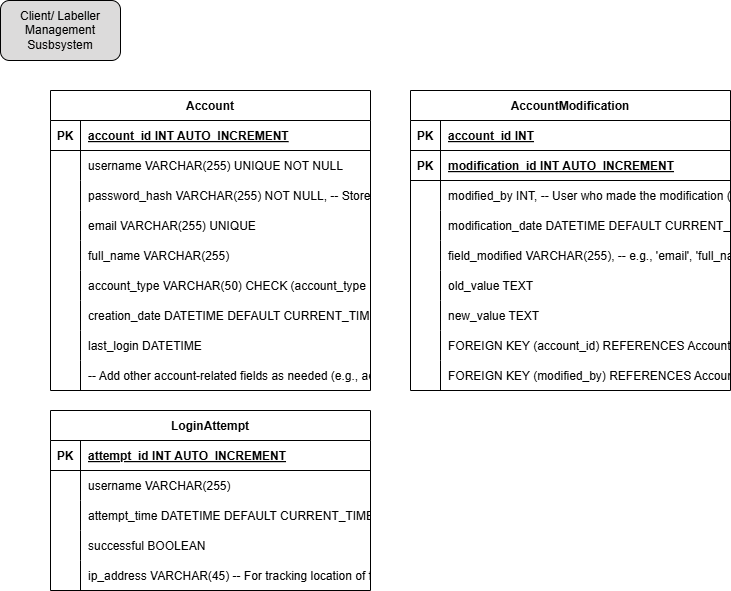
\includegraphics[scale=0.5]{dt2.png}\\
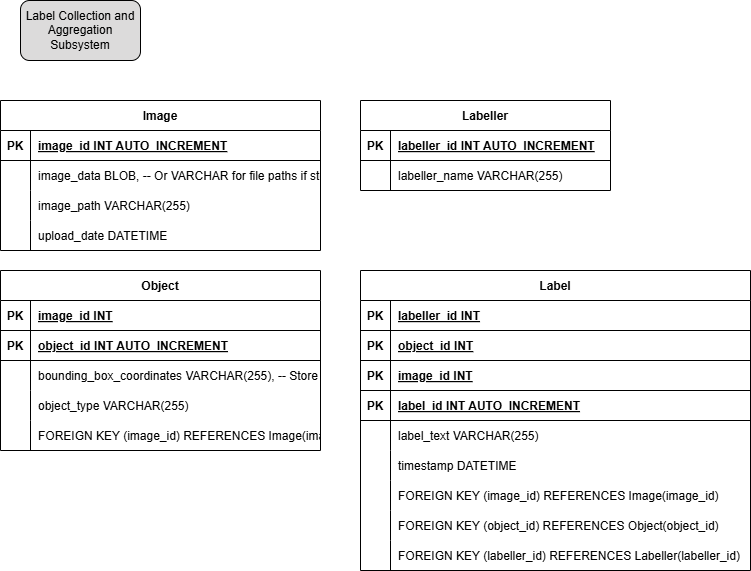
\includegraphics[scale=0.5]{dt5.png}\\

\newpage 
\section{Module Decomposition}

The following table is taken directly from the Module Guide document for this project.

\begin{table}[h!]
  \centering
  \begin{tabular}{p{0.3\textwidth} p{0.6\textwidth}}
  \toprule
  \textbf{Level 1} & \textbf{Level 2}\\
  \midrule
  
  \textbf{Hardware-Hiding Module} & ~ \\
  \midrule
\end{tabular}
\caption{Module Hierarchy}
\label{TblMH}
\end{table}
\begin{table}[h!]
  \centering
  \begin{tabular}{p{0.3\textwidth} p{0.6\textwidth}}
  \toprule
  \textbf{Level 1} & \textbf{Level 2}\\
  \multirow{10}{0.3\textwidth}{\textbf{Behaviour-Hiding Module}} 
   & Account Creation Interface\\
   & Account Database\\
   & Account Update Interface\\
   & Login Interface\\
   & Access Token\\
   & Labeler\\
   & Client\\
   & User\\
   & Satellite Image Request Interface\\
   & Satellite Image Request\\
   & Project Creation Interface\\
   & Project\\
   & Service Request Failure Interface\\
   & Image Upload Interface\\
   & Report Interface\\
   & Report\\
   & Project Selection Interface\\
   & Labeling Interface\\
   & Image\\
   & Label Server\\
   & Label Database Connector\\
   & Label Database\\
   & ImageObject Database Connector\\
   & ImageObject Database\\
   & Labeller Database Connector\\
   & Labeller Database\\
   & Object Extraction Manager\\
   & Image Service Manager\\
   % New ML/Model modules (Behavior-Hiding)
   & ModelCreation (Abstract Class)\\
   & CNNModelCreation\\
   & OtherModelCreation\\
   & ModelManager\\
   & MLModelDatabase\\
  \midrule
\end{tabular}
\caption{Module Hierarchy}
\label{TblMH}
\end{table}
\begin{table}[h!]
  \centering
  \begin{tabular}{p{0.3\textwidth} p{0.6\textwidth}}
  \toprule
  \textbf{Level 1} & \textbf{Level 2}\\
  \multirow{10}{0.3\textwidth}{\textbf{Software Decision Module}} 
   & Account Creation Controller\\
   & Account Database Connector\\
   & Account Update Controller\\
   & Authentication Controller\\
   & Satellite Image Request Controller\\
   & Project Creation Controller\\
   & Report Controller\\
   & Project Selection Controller\\
   & Labeling Controller\\
   & Label Confidence Service\\
   & Object Extraction Service\\
   & Image Prior Analyzer\\
   & Labeller Expertise Calculator\\
   & Image Mask Service\\
   & Image Selection Service\\
   % New ML/Model modules (Software Decision)
   & ModelComparision Evaluation\\
   & CrossValidation Evaluation\\
   & ModelTrainingService\\
   & ModelEvaluationService\\
  \bottomrule
  \end{tabular}
  \caption{Module Hierarchy}
  \label{TblMH}
  \end{table}
  

\newpage 

~\newpage 

% \section{MIS of \wss{Module Name}} \label{Module} \wss{Use labels for
%   cross-referencing}

% \wss{You can reference SRS labels, such as R\ref{R_Inputs}.}

% \wss{It is also possible to use \LaTeX for hypperlinks to external documents.}

% \subsection{Module}

% \wss{Short name for the module}

% \subsection{Uses}


% \subsection{Syntax}

% \subsubsection{Exported Constants}

% \subsubsection{Exported Access Programs}

% \begin{center}
% \begin{tabular}{p{2cm} p{4cm} p{4cm} p{2cm}}
% \hline
% \textbf{Name} & \textbf{In} & \textbf{Out} & \textbf{Exceptions} \\
% \hline
% \wss{accessProg} & - & - & - \\
% \hline
% \end{tabular}
% \end{center}

% \subsection{Semantics}

% \subsubsection{State Variables}

% \wss{Not all modules will have state variables.  State variables give the module
%   a memory.}

% \subsubsection{Environment Variables}

% \wss{This section is not necessary for all modules.  Its purpose is to capture
%   when the module has external interaction with the environment, such as for a
%   device driver, screen interface, keyboard, file, etc.}

% \subsubsection{Assumptions}

% \wss{Try to minimize assumptions and anticipate programmer errors via
%   exceptions, but for practical purposes assumptions are sometimes appropriate.}

% \subsubsection{Access Routine Semantics}

% \noindent \wss{accessProg}():
% \begin{itemize}
% \item transition: \wss{if appropriate} 
% \item output: \wss{if appropriate} 
% \item exception: \wss{if appropriate} 
% \end{itemize}

% \wss{A module without environment variables or state variables is unlikely to
%   have a state transition.  In this case a state transition can only occur if
%   the module is changing the state of another module.}

% \wss{Modules rarely have both a transition and an output.  In most cases you
%   will have one or the other.}


% OG
\section{MIS of Report Manager} \label{rm} 
    \subsection{Module}
        RM (ReportManager)

    \subsection{Uses}
        LabelDBConnector \ref{label database connector}\\
        ObjectsOnImageDBConnector \ref{ImageObject database connector}\\
        RawImageDBConnector \ref{cidbc}\\
        ProjectDBConnector \ref{pdbc}

    \subsection{Syntax}
    \subsubsection{Exported Constants}
        None

    \subsubsection{Exported Access Programs}
    \begin{center}\begin{tabular}{p{3cm} p{4cm} p{3cm} p{3cm}}
    \hline\textbf{Name} & \textbf{In} & \textbf{Out} & \textbf{Exceptions} \\
    \hline
        generateReport & projectId: String & Report & DatabaseException \\
    \hline
    \end{tabular}\end{center}

    \subsection{Semantics}
    \subsubsection{State Variables}
        None

    \subsubsection{Environment Variables}
        None

    \subsubsection{Assumptions}
        None

    \subsubsection{Access Routine Semantics}
        \noindent generateReport(projectId: String)
        \begin{itemize}
            \item output: Returns a Report object that aggregates data from the label, object-on-image, raw image, and project databases.
            \item exception: DatabaseException: Thrown if there is an issue communicating with any of the underlying databases.
        \end{itemize}

    \subsubsection{Local Functions}
        Any helper methods used internally to combine or transform the data (e.g., formatting label lists, summarizing object data) are not exported and thus not specified here.


  
\section{MIS of Account Creation Interface} \label{aci}

\subsection{Module}

Account Creation Interface

\subsection{Uses}

Account Creation Controller \ref{acc}

\subsection{Syntax}

\subsubsection{Exported Constants}
None
\subsubsection{Exported Access Programs}

\begin{center}
\begin{tabular}{p{2cm} p{4cm} p{4cm} p{2cm}}
\hline
\textbf{Name} & \textbf{In} & \textbf{Out} & \textbf{Exceptions} \\
\hline
renderPage & Enum[labeler, client] & - & - \\
submitForm & list[(string, string)] & - & - \\
\hline
\end{tabular}
\end{center}

\subsection{Semantics}

\subsubsection{State Variables}
None
\subsubsection{Environment Variables}
win: 2D sequence of coloured pixels

\subsubsection{Assumptions}
None

\subsubsection{Access Routine Semantics}

\noindent renderPage(userType):
\begin{itemize}
\item transition: win := Modify window so that it shows a registration form that asks for the necessary information depending on if the user is a labeler or client.
\end{itemize}

\noindent submitForm(formData):
\begin{itemize}
\item transition: Passes the submitted form data to the Account Creation Controller for validation and processing.
\end{itemize}

\subsubsection{Local Functions}
None




% OG
\section{MIS of Project Manager} \label{pm} 
    \subsection{Module}
        PM (ProjectManager)

    \subsection{Uses}
        ProjectCollectionManager \ref{pcm}\\
        CoreImageDBConnector \ref{cidbc}

    \subsection{Syntax}
    \subsubsection{Exported Constants}
        None

    \subsubsection{Exported Access Programs}
    \begin{center}\begin{tabular}{p{3cm} p{4cm} p{3cm} p{3cm}}
    \hline\textbf{Name} & \textbf{In} & \textbf{Out} & \textbf{Exceptions} \\
    \hline
        createProject & projectName: String, metadata: Map(String, String) & Project & DatabaseException \\
        addImageToProject & projectId: String, byte[] & void & DatabaseException \\
    \hline
    \end{tabular}\end{center}

    \subsection{Semantics}
    \subsubsection{State Variables}
        None

    \subsubsection{Environment Variables}
        None

    \subsubsection{Assumptions}
        None

    \subsubsection{Access Routine Semantics}
        \noindent createProject(projectName, metadata)
        \begin{itemize}
            \item output: Returns a newly created Project object with a unique identifier and any associated metadata.
            \item exception: \textbf{ProjectAlreadyExistsException}: Thrown if a project with the same name or identifier already exists. \textbf{DatabaseException}: Thrown if any error occurs while writing to the database.
        \end{itemize}
        \noindent addImageToProject(projectId, imageData)
        \begin{itemize}
            \item exception: \textbf{InvalidImageException}: Thrown if the image data is corrupted or unsupported. \textbf{ProjectNotFoundException}: Thrown if the target project does not exist in the system. \textbf{DatabaseException}: Thrown if a database error occurs while storing the image.
        \end{itemize}

    \subsubsection{Local Functions}
        Internal helper methods (e.g., validation, transformations) are not exported.

% OG
\section{MIS of Project Collection Manager} \label{pcm} 
    \subsection{Module}
        PCM (ProjectCollectionManager)

    \subsection{Uses}
        ProjectDBConnector \ref{pdbc}

    \subsection{Syntax}
    \subsubsection{Exported Constants}
        None

    \subsubsection{Exported Access Programs}
    \begin{center}\begin{tabular}{p{3cm} p{3cm} p{3cm} p{3cm}}
    \hline\textbf{Name} & \textbf{In} & \textbf{Out} & \textbf{Exceptions} \\
    \hline
        getAvailableProjects & None & List(Project) & DatabaseException \\
    \hline
    \end{tabular}\end{center}

    \subsection{Semantics}
    \subsubsection{State Variables}
        None

    \subsubsection{Environment Variables}
        None

    \subsubsection{Assumptions}
        None

    \subsubsection{Access Routine Semantics}
        \noindent getAvailableProjects()
        \begin{itemize}
            \item output: Returns a list of existing Project objects (could be filtered by user permissions or some criteria, if applicable).
            \item exception: \textbf{ProjectAlreadyExistsException}: Thrown if a project with the same name or identifier already exists. 
        \end{itemize}
    \subsubsection{Local Functions}
        Internal helper methods (e.g., transformations) are not exported.



% OG
\section{MIS of Project Database Connector} \label{pdbc} 
    \subsection{Module}
        PDBC (ProjectDBConnector)

    \subsection{Uses}
        MySQL - ProjectDB

    \subsection{Syntax}
    \subsubsection{Exported Constants}
        None

    \subsubsection{Exported Access Programs}
    \begin{center}\begin{tabular}{p{3cm} p{4cm} p{3cm} p{3cm}}
    \hline\textbf{Name} & \textbf{In} & \textbf{Out} & \textbf{Exceptions} \\
    \hline
        fetchProject & projectId: String & Project & DatabaseException \\
        fetchProjectList & None & List(Project) & DatabaseException \\
        storeProject & project : Project & None & DatabaseException \\
    \hline
    \end{tabular}\end{center}

    \subsection{Semantics}
    \subsubsection{State Variables}
        None

    \subsubsection{Environment Variables}
        databaseConnection: connection to relational database

    \subsubsection{Assumptions}
        None

    \subsubsection{Access Routine Semantics}
        \noindent storeProject(project : Project)
        \begin{itemize}
            \item output: No direct output; success indicates the Project was successfully stored.
            \item exception: \textbf{DatabaseException}: Thrown if there is an issue communicating with any of the underlying databases. \textbf{DuplicateProjectException}: Thrown if the project already exists
        \end{itemize}
        \noindent fetchProjectList()
        \begin{itemize}
            \item output: Returns a list of all Project objects stored in the database.
            \item exception: \textbf{DatabaseException}: Thrown if there is an issue communicating with any of the underlying databases. 
        \end{itemize}
        \noindent fetchProject(projectId : String)
        \begin{itemize}
            \item output: Returns the Project object corresponding to the given projectId.
            \item exception: \textbf{DatabaseException}: Thrown if there is an issue communicating with any of the underlying databases. \textbf{ProjectNotFoundException}: Thrown if the project with the given ID does not exist.
        \end{itemize}

    \subsubsection{Local Functions}
        Any database query-building or data-mapping helpers remain internal and are not exported.

% OG
\section{MIS of Core Image Database Connector} \label{cidbc}
    \subsection{Module}
        CIDBC (CoreImageDBConnector)

    \subsection{Uses}
        MySQL - CoreImageDB

    \subsection{Syntax}
    \subsubsection{Exported Constants}
        None

    \subsubsection{Exported Access Programs}
    \begin{center}\begin{tabular}{p{3cm} p{4cm} p{3cm} p{3cm}}
    \hline\textbf{Name} & \textbf{In} & \textbf{Out} & \textbf{Exceptions} \\
    \hline
        storeImage & projectId: String imageData: byte[] & String & DatabaseException \\
        fetchImage & imageId: String & Image & DatabaseException \\
        fetchImageForProject & projectId: String & List(Image) & DatabaseException \\
    \hline
    \end{tabular}\end{center}

    \subsection{Semantics}
    \subsubsection{State Variables}
        None

    \subsubsection{Environment Variables}
        databaseConnection: connection to relational database

    \subsubsection{Assumptions}
        None

    \subsubsection{Access Routine Semantics}
        \noindent storeImage(projectId, imageData)
        \begin{itemize}
            \item output: Returns a newly generated String identifier (imageId) that uniquely identifies the stored image in the database.
            \item exception: \textbf{DatabaseException}: Thrown if there is an issue communicating with any of the underlying databases. \textbf{ProjectNotFoundException}: Thrown if the specified projectId does not exist in the database.
        \end{itemize}
        \noindent fetchImage(imageId)
        \begin{itemize}
            \item output: Returns an Image object (or equivalent data structure) for the given imageId, including any relevant metadata or binary content.
            \item exception: \textbf{DatabaseException}: Thrown if there is an issue communicating with any of the underlying databases. 
            \textbf{ImageNotFoundException}: Thrown if no image with the specified imageId exists in the database.
        \end{itemize}
        \noindent fetchImagesForProject(projectId)
        \begin{itemize}
            \item output: Returns a list of Image objects associated with the specified projectId.
            \item exception: \textbf{DatabaseException}: Thrown if there is an issue communicating with any of the underlying databases. \textbf{ProjectNotFoundException}: Thrown if the project with the given ID does not exist.
        \end{itemize}
    \subsubsection{Local Functions}
        Any database query-building or data-mapping helpers remain internal and are not exported.




\section{MIS of Account Database Connector} \label{accdc}

\subsection{Module}

Account Database Connector

\subsection{Uses}

Account Database \ref{accd}

\subsection{Syntax}

\subsubsection{Exported Constants}
None
\subsubsection{Exported Access Programs}

\begin{center}
\begin{tabular}{p{2cm} p{4cm} p{4cm} p{2cm}}
\hline
\textbf{Name} & \textbf{In} & \textbf{Out} & \textbf{Exceptions} \\
\hline
insertUser & User & - & - \\
retrieveUser & string & User & - \\
updateUser & User & - & - \\
userExists & string & boolean & - \\
makeDBConnection & credentials & & - \\
\hline
\end{tabular}
\end{center}

\subsection{Semantics}

\subsubsection{State Variables}
None
\subsubsection{Environment Variables}
databaseConnection: connection to relational database

\subsubsection{Assumptions}
None

\subsubsection{Access Routine Semantics}

\noindent insertUser(user):
\begin{itemize}
\item transition: Request to insert user into database through databaseConection.
\end{itemize}

\noindent retrieveUser(email):
\begin{itemize}
\item output: 
\[
\begin{cases}
    \text{User where User.email == email}, & \text{if } \text{userExists(email)}\\
    \text{null}, & \text{otherwise}
\end{cases}
\]
\end{itemize}

\noindent updateUser(user):
\begin{itemize}
\item transition: 
\[
\begin{cases}
    \text{Request to update user in database}, & \text{if } \text{userExists(user.email)}\\
    \text{Do nothing} & \text{otherwise}
\end{cases}
\]
\end{itemize}

\noindent userExists(email):
\begin{itemize}
\item output: out := 
\[ \exists \, \text{User} \in \text{Database} \, \text{s.t.} \, \text{User.email} == \text{email}
\]
\end{itemize}

\noindent makeDBConnection(credentials):
\begin{itemize}
\item transition: databaseConnection := connection is established with database if credentials are correct
\end{itemize}


\subsubsection{Local Functions}
None

\section{MIS of Account Database} \label{accd}

\subsection{Module}

Account Database

\subsection{Uses}

None

\subsection{Syntax}

\subsubsection{Exported Constants}
None
\subsubsection{Exported Access Programs}

\begin{center}
\begin{tabular}{p{2cm} p{4cm} p{4cm} p{2cm}}
\hline
\textbf{Name} & \textbf{In} & \textbf{Out} & \textbf{Exceptions} \\
\hline
insertUser & User & - & - \\
retrieveUser & string & User & - \\
updateUser & User & - & - \\
userExists & string & boolean & - \\
\hline
\end{tabular}
\end{center}

\subsection{Semantics}

\subsubsection{State Variables}
None
\subsubsection{Environment Variables}
databaseConnection: connection to Application

\subsubsection{Assumptions}
None

\subsubsection{Access Routine Semantics}

\noindent insertUser(user):
\begin{itemize}
\item transition: Insert user into database.
\end{itemize}

\noindent retrieveUser(email):
\begin{itemize}
\item output: 
\[
\begin{cases}
    \text{User where User.email == email}, & \text{if } \text{userExists(email)}\\
    \text{null}, & \text{otherwise}
\end{cases}
\]
\end{itemize}

\noindent updateUser(user):
\begin{itemize}
\item transition: 
\[
\begin{cases}
    \text{Update user in database}, & \text{if } \text{userExists(user.email)}\\
    \text{Do nothing} & \text{otherwise}
\end{cases}
\]
\end{itemize}

\noindent userExists(email):
\begin{itemize}
\item output: out := 
\[ \exists \, \text{User} \in \text{Database} \, \text{s.t.} \, \text{User.email} == \text{email}
\]
\end{itemize}


\subsubsection{Local Functions}
None

\section{MIS of Account Update Interface} \label{aui}

\subsection{Module}

Account Update Interface

\subsection{Uses}

Account Update Controller \ref{auc}

\subsection{Syntax}

\subsubsection{Exported Constants}
None
\subsubsection{Exported Access Programs}

\begin{center}
\begin{tabular}{p{2cm} p{4cm} p{4cm} p{2cm}}
\hline
\textbf{Name} & \textbf{In} & \textbf{Out} & \textbf{Exceptions} \\
\hline
renderPage & User & - & - \\
submitForm & list[(string, string)] & - & - \\
\hline
\end{tabular}
\end{center}

\subsection{Semantics}

\subsubsection{State Variables}
None
\subsubsection{Environment Variables}
win: 2D sequence of coloured pixels

\subsubsection{Assumptions}
None

\subsubsection{Access Routine Semantics}

\noindent renderPage(userInfo):
\begin{itemize}
\item transition: win := Modify window so that it shows a form with the current user's information. This information can be changed by the user.
\end{itemize}

\noindent submitForm(formData):
\begin{itemize}
\item transition: Passes the submitted changes to the Account Update Controller for validation and processing.
\end{itemize}

\subsubsection{Local Functions}
None

\section{MIS of Login Interface} \label{li}

\subsection{Module}

Login Interface

\subsection{Uses}

Authentication Controller \ref{ac}

\subsection{Syntax}

\subsubsection{Exported Constants}
None
\subsubsection{Exported Access Programs}

\begin{center}
\begin{tabular}{p{2cm} p{4cm} p{4cm} p{2cm}}
\hline
\textbf{Name} & \textbf{In} & \textbf{Out} & \textbf{Exceptions} \\
\hline
renderPage & - & - & - \\
submitForm & list[(string, string)] & - & - \\
\hline
\end{tabular}
\end{center}

\subsection{Semantics}

\subsubsection{State Variables}
None
\subsubsection{Environment Variables}
win: 2D sequence of coloured pixels

\subsubsection{Assumptions}
None

\subsubsection{Access Routine Semantics}

\noindent renderPage():
\begin{itemize}
\item transition: win := Modify window so that it shows a login form.
\end{itemize}

\noindent submitForm(formData):
\begin{itemize}
\item transition: Passes the submitted credentials to the Authentication Controller for validation.
\end{itemize}

\subsubsection{Local Functions}
None

\section{MIS of Access Token} \label{at}

\subsection{Module}

Access Token

\subsection{Uses}
None

\subsection{Syntax}

\subsubsection{Exported Constants}
None
\subsubsection{Exported Access Programs}

\begin{center}
\begin{tabular}{p{2cm} p{4cm} p{4cm} p{2cm}}
\hline
\textbf{Name} & \textbf{In} & \textbf{Out} & \textbf{Exceptions} \\
\hline
isExpired & - & boolean & - \\
renew & - & - & - \\
\hline
\end{tabular}
\end{center}

\subsection{Semantics}

\subsubsection{State Variables}
\begin{itemize}
    \item tokenValue: string
    \item expirationTime: Date
    \item userID: string
\end{itemize}
\subsubsection{Environment Variables}
None

\subsubsection{Assumptions}
None

\subsubsection{Access Routine Semantics}

\noindent isExpired():
\begin{itemize}
\item output: out := currentTime $>$ expirationTime
\end{itemize}

\noindent renew():
\begin{itemize}
\item transition: expirationTime := expirationTime + 5 hours
\end{itemize}

\subsubsection{Local Functions}
None

\section{MIS of Account Creation Interface} \label{aci}

\subsection{Module}

Account Creation Interface

\subsection{Uses}

Account Creation Controller \ref{acc}

\subsection{Syntax}

\subsubsection{Exported Constants}
None
\subsubsection{Exported Access Programs}

\begin{center}
\begin{tabular}{p{2cm} p{4cm} p{4cm} p{2cm}}
\hline
\textbf{Name} & \textbf{In} & \textbf{Out} & \textbf{Exceptions} \\
\hline
renderPage & Enum[labeler, client] & - & - \\
submitForm & list[(string, string)] & - & - \\
\hline
\end{tabular}
\end{center}

\subsection{Semantics}

\subsubsection{State Variables}
None
\subsubsection{Environment Variables}
win: 2D sequence of coloured pixels

\subsubsection{Assumptions}
None

\subsubsection{Access Routine Semantics}

\noindent renderPage(userType):
\begin{itemize}
\item transition: win := Modify window so that it shows a registration form that asks for the necessary information depending on if the user is a labeler or client.
\end{itemize}

\noindent submitForm(formData):
\begin{itemize}
\item transition: Passes the submitted form data to the Account Creation Controller for validation and processing.
\end{itemize}

\subsubsection{Local Functions}
None

\section{MIS of Account Database} \label{accd}

\subsection{Module}

Account Database

\subsection{Uses}

Relational Database

\subsection{Syntax}

\subsubsection{Exported Constants}
None
\subsubsection{Exported Access Programs}

\begin{center}
\begin{tabular}{p{2cm} p{4cm} p{4cm} p{2cm}}
\hline
\textbf{Name} & \textbf{In} & \textbf{Out} & \textbf{Exceptions} \\
\hline
insertUser & User & - & - \\
retrieveUser & string & User & - \\
updateUser & User & - & - \\
userExists & string & boolean & - \\
\hline
\end{tabular}
\end{center}

\subsection{Semantics}

\subsubsection{State Variables}
None
\subsubsection{Environment Variables}
databaseConnection: connection to relational database

\subsubsection{Assumptions}
None

\subsubsection{Access Routine Semantics}

\noindent insertUser(user):
\begin{itemize}
\item transition: Insert user into database through databaseConection.
\end{itemize}

\noindent retrieveUser(email):
\begin{itemize}
\item output: 
\[
\begin{cases}
    \text{User where User.email == email}, & \text{if } \text{userExists(email)}\\
    \text{null}, & \text{otherwise}
\end{cases}
\]
\end{itemize}

\noindent updateUser(user):
\begin{itemize}
\item transition: 
\[
\begin{cases}
    \text{Update user in database through databaseConection}, & \text{if } \text{userExists(user.email)}\\
    \text{Do nothing} & \text{otherwise}
\end{cases}
\]
\end{itemize}

\noindent userExists(email):
\begin{itemize}
\item output: out := 
\[ \exists \, \text{User} \in \text{Database} \, \text{s.t.} \, \text{User.email} = \text{email}
\]
\end{itemize}


\subsubsection{Local Functions}
None

\section{MIS of Account Update Interface} \label{aui}

\subsection{Module}

Account Update Interface

\subsection{Uses}

Account Update Controller \ref{auc}

\subsection{Syntax}

\subsubsection{Exported Constants}
None
\subsubsection{Exported Access Programs}

\begin{center}
\begin{tabular}{p{2cm} p{4cm} p{4cm} p{2cm}}
\hline
\textbf{Name} & \textbf{In} & \textbf{Out} & \textbf{Exceptions} \\
\hline
renderPage & User & - & - \\
submitForm & list[(string, string)] & - & - \\
\hline
\end{tabular}
\end{center}

\subsection{Semantics}

\subsubsection{State Variables}
None
\subsubsection{Environment Variables}
win: 2D sequence of coloured pixels

\subsubsection{Assumptions}
None

\subsubsection{Access Routine Semantics}

\noindent renderPage(userInfo):
\begin{itemize}
\item transition: win := Modify window so that it shows a form with the current user's information. This information can be changed by the user.
\end{itemize}

\noindent submitForm(formData):
\begin{itemize}
\item transition: Passes the submitted changes to the Account Update Controller for validation and processing.
\end{itemize}

\subsubsection{Local Functions}
None

\section{MIS of Login Interface} \label{li}

\subsection{Module}

Login Interface

\subsection{Uses}

Authentication Controller \ref{ac}

\subsection{Syntax}

\subsubsection{Exported Constants}
None
\subsubsection{Exported Access Programs}

\begin{center}
\begin{tabular}{p{2cm} p{4cm} p{4cm} p{2cm}}
\hline
\textbf{Name} & \textbf{In} & \textbf{Out} & \textbf{Exceptions} \\
\hline
renderPage & - & - & - \\
submitForm & list[(string, string)] & - & - \\
\hline
\end{tabular}
\end{center}

\subsection{Semantics}

\subsubsection{State Variables}
None
\subsubsection{Environment Variables}
win: 2D sequence of coloured pixels

\subsubsection{Assumptions}
None

\subsubsection{Access Routine Semantics}

\noindent renderPage():
\begin{itemize}
\item transition: win := Modify window so that it shows a login form.
\end{itemize}

\noindent submitForm(formData):
\begin{itemize}
\item transition: Passes the submitted credentials to the Authentication Controller for validation.
\end{itemize}

\subsubsection{Local Functions}
None

\section{MIS of Access Token} \label{at}

\subsection{Module}

Access Token

\subsection{Uses}
None

\subsection{Syntax}

\subsubsection{Exported Constants}
None
\subsubsection{Exported Access Programs}

\begin{center}
\begin{tabular}{p{2cm} p{4cm} p{4cm} p{2cm}}
\hline
\textbf{Name} & \textbf{In} & \textbf{Out} & \textbf{Exceptions} \\
\hline
isExpired & - & boolean & - \\
renew & - & - & - \\
\hline
\end{tabular}
\end{center}

\subsection{Semantics}

\subsubsection{State Variables}
\begin{itemize}
    \item tokenValue: string
    \item expirationTime: Date
    \item userID: string
\end{itemize}
\subsubsection{Environment Variables}
None

\subsubsection{Assumptions}
None

\subsubsection{Access Routine Semantics}

\noindent isExpired():
\begin{itemize}
\item output: out := currentTime $>$ expirationTime
\end{itemize}

\noindent renew():
\begin{itemize}
\item transition: expirationTime := expirationTime + 5 hours
\end{itemize}

\subsubsection{Local Functions}
None

\section{MIS of Labeler} \label{labeler}

\subsection{Module}

Labeler

\subsection{Uses}
Extends User \ref{user}

\subsection{Syntax}

\subsubsection{Exported Constants}
None
\subsubsection{Exported Access Programs}

\begin{center}
\begin{tabular}{p{3cm} p{4cm} p{4cm} p{2cm}}
\hline
\textbf{Name} & \textbf{In} & \textbf{Out} & \textbf{Exceptions} \\
\hline
getFirstName & - & string & - \\
getLastName & - & string & - \\
getSkills & - & list[string] & - \\
getAvailability & - & int & - \\
setFirstName & string & - & - \\
setLastName & string & - & - \\
setSkills & list[string] & - & - \\
setAvailability & int & - & - \\
\hline
\end{tabular}
\end{center}

\subsection{Semantics}

\subsubsection{State Variables}
\begin{itemize}
    \item firstName: string
    \item lastName: string
    \item skills: list[string]
    \item availability: int
\end{itemize}
\subsubsection{Environment Variables}
None

\subsubsection{Assumptions}
None

\subsubsection{Access Routine Semantics}

\noindent getFirstName():
\begin{itemize}
\item output: out := firstName
\end{itemize}

\noindent getLastName():
\begin{itemize}
\item output: out := lastName
\end{itemize}

\noindent getSkills():
\begin{itemize}
\item output: out := skills
\end{itemize}

\noindent getAvailability():
\begin{itemize}
\item output: out := availability
\end{itemize}

\noindent setFirstName(newfn):
\begin{itemize}
\item transition: firstName := newfn 
\end{itemize}

\noindent setLastName(newln):
\begin{itemize}
\item transition: lastName := newln
\end{itemize}

\noindent setSkills(newSkills):
\begin{itemize}
\item transition: skills := newSkills 
\end{itemize}

\noindent setAvailability(newAvail):
\begin{itemize}
\item transition: availability := newAvail
\end{itemize}

\subsubsection{Local Functions}
None

\section{MIS of Client} \label{client}

\subsection{Module}

Client

\subsection{Uses}
Extends User \ref{user}

\subsection{Syntax}

\subsubsection{Exported Constants}
None
\subsubsection{Exported Access Programs}

\begin{center}
\begin{tabular}{p{3.2cm} p{4cm} p{4cm} p{2cm}}
\hline
\textbf{Name} & \textbf{In} & \textbf{Out} & \textbf{Exceptions} \\
\hline
getCompanyName & - & string & - \\
getIndustry & - & string & - \\
getTypicalProject & - & Image & - \\
setCompanyName & string & - & - \\
setIndustry & string & - & - \\
setTypicalProject & string & - & - \\
\hline
\end{tabular}
\end{center}

\subsection{Semantics}

\subsubsection{State Variables}
\begin{itemize}
    \item companyName: string
    \item industry: string
    \item typicalProject: string
\end{itemize}
\subsubsection{Environment Variables}
None

\subsubsection{Assumptions}
None

\subsubsection{Access Routine Semantics}

\noindent getCompanyName():
\begin{itemize}
\item output: out := companyName
\end{itemize}

\noindent getIndustry():
\begin{itemize}
\item output: out := industry
\end{itemize}

\noindent getTypicalProject():
\begin{itemize}
\item output: out := typicalProject
\end{itemize}

\noindent setCompanyName(newcn):
\begin{itemize}
\item transition: companyName := newcn 
\end{itemize}

\noindent setIndustry(newIndustry):
\begin{itemize}
\item transition: industry := newIndustry
\end{itemize}

\noindent setTypicalProject(newtp):
\begin{itemize}
\item transition: typicalProject := newtp 
\end{itemize}

\subsubsection{Local Functions}
None

\section{MIS of User} \label{user}

\subsection{Module}

User

\subsection{Uses}
None

\subsection{Syntax}

\subsubsection{Exported Constants}
None
\subsubsection{Exported Access Programs}

\begin{center}
\begin{tabular}{p{2cm} p{4cm} p{4cm} p{2cm}}
\hline
\textbf{Name} & \textbf{In} & \textbf{Out} & \textbf{Exceptions} \\
\hline
getEmail & - & string & - \\
getPassword & - & string & - \\
getProfilePic & - & Image & - \\
setEmail & string & - & - \\
setPassword & string & - & - \\
setProfilePic & string & - & - \\
\hline
\end{tabular}
\end{center}

\subsection{Semantics}

\subsubsection{State Variables}
\begin{itemize}
    \item email: string
    \item password: string
    \item profilePic: image
\end{itemize}
\subsubsection{Environment Variables}
None

\subsubsection{Assumptions}
None

\subsubsection{Access Routine Semantics}

\noindent getEmail():
\begin{itemize}
\item output: out := email
\end{itemize}

\noindent getPassword():
\begin{itemize}
\item output: out := password
\end{itemize}

\noindent getProfilePic():
\begin{itemize}
\item output: out := profilePic
\end{itemize}

\noindent setEmail(newEmail):
\begin{itemize}
\item transition: email := newEmail 
\end{itemize}

\noindent setPassword(newPassword):
\begin{itemize}
\item transition: password := newPassword
\end{itemize}

\noindent setProfilePic(newProfliePic):
\begin{itemize}
\item transition: profilePic := newProfilePic 
\end{itemize}

\subsubsection{Local Functions}
None

\section{MIS of Account Creation Controller} \label{acc}

\subsection{Module}

Account Creation Controller

\subsection{Uses}

Account Creation Interface \ref{aci}\\
Account Database \ref{accd} \\
User \ref{user} \\
Labeler \ref{labeler} \\
Client \ref{client}

\subsection{Syntax}

\subsubsection{Exported Constants}
None
\subsubsection{Exported Access Programs}

\begin{center}
\begin{tabular}{p{2cm} p{4cm} p{4cm} p{2cm}}
\hline
\textbf{Name} & \textbf{In} & \textbf{Out} & \textbf{Exceptions} \\
\hline
validateForm & list[(string, string)], Enum[labeler, client] & boolean & - \\
createUser & list[(string, string)], Enum[labeler, client] & User & - \\
uploadUser & User & - & DatabaseException \\
\hline
\end{tabular}
\end{center}

\subsection{Semantics}

\subsubsection{State Variables}
None

\subsubsection{Environment Variables}
None

\subsubsection{Assumptions}
Assumes AccountDatabase is operational when calling uploadUser.

\subsubsection{Access Routine Semantics}
\noindent validateForm(formData, userType):
\begin{itemize}
\item output: out := 
$ \text{hasRequiredFields}(\text{formData}, \text{userFields}) \land \nonumber
    \text{isValidEmail}(\text{formData.email}) \land \nonumber \\
    \text{isValidPassword}(\text{formData.password}) \land $
\[
\begin{cases}
    \text{hasRequiredFields}(\text{formData}, \text{labelerFields}), & \text{if } \text{userType} = \text{"labeler"} \\
    \text{hasRequiredFields}(\text{formData}, \text{clientFields}), & \text{if } \text{userType} = \text{"client"} \\
    \text{true}, & \text{otherwise}
\end{cases}
\]
\textbf{Where:}
\begin{align*}
    \text{userFields} &= \{ \text{email, password} \} \\
    \text{labelerFields} &= \{ \text{firstName, lastName, skills, availability} \} \\
    \text{clientFields} &= \{ \text{companyName, industry, typicalProject} \}
\end{align*}
\end{itemize}

\noindent createUser(formData, userType):
\begin{itemize}
\item output: out := 
\[
\begin{cases}
    \text{Labeler}(\text{formData.email}, \text{formData.password}, \text{formData.firstName}, \\ \text{formData.lastName}, \text{formData.skills}, \text{int(formData.availability)}), & \text{if } \text{userType} = \text{"labeler"} \\
    \text{Client}(\text{formData.email}, \text{formData.password}, \text{formData.companyName}, \\ \text{formData.industry}, \text{formData.typicalProject}) & \text{if } \text{userType} = \text{"client"} \\
\end{cases}
\]
\end{itemize}

\noindent uploadUser(newUser):
\begin{itemize}
\item transition: Passes the User object to the AccountDatabase for storage.
\item exception: Throws DatabaseException if storage fails.
\end{itemize}

\subsubsection{Local Functions}
\begin{itemize}
    \item 
        \text{hasRequiredFields}(\text{data}, \text{fields}) =
        $\forall \text{field} \in \text{fields}, (\text{data[field]} \neq \text{""})$
        
    \item isValidEmail(email) = $\text{email} \in V \land \text{email} \neg \in \text{Registered Emails}$
    
    Let E represent the set of all email addresses, and let V represent the set of all valid email addresses. A valid email address conforms to the general pattern:\\\\
  V = $(\forall\; email \in E\;  |\; email \; matches \; the \; pattern \; $[a-zA-Z0-9+\_.-]+@[a-zA-Z0-9.-]+[a-zA-Z])
  \item isValidPassword(password) = $(password \; matches \; the \; pattern \; $(?=.*[a-z])(?=.*[A-Z])(?=.*[0-9])(?=.*[\#\$\%\&\*\@])[a-zA-Z0-9\#\$\%\&\*\@]\{8,\})\\
  
\end{itemize}

\section{MIS of Account Update Controller} \label{auc}

\subsection{Module}

Account Update Controller

\subsection{Uses}

Account Update Interface \ref{aui}\\
Account Database \ref{accd} \\
User \ref{user} \\

\subsection{Syntax}

\subsubsection{Exported Constants}
None
\subsubsection{Exported Access Programs}

\begin{center}
\begin{tabular}{p{3cm} p{4cm} p{4cm} p{2cm}}
\hline
\textbf{Name} & \textbf{In} & \textbf{Out} & \textbf{Exceptions} \\
\hline
validateForm & list[(string, string)] & boolean & - \\
getUser & string & - & - \\
requestUpdate & User & - & DatabaseException \\
\hline
\end{tabular}
\end{center}

\subsection{Semantics}

\subsubsection{State Variables}
\begin{itemize}
    \item user: User
\end{itemize}

\subsubsection{Environment Variables}
None

\subsubsection{Assumptions}
Assumes AccountDatabase is operational when calling requestUpdate.

\subsubsection{Access Routine Semantics}
\noindent validateForm(formData):
\begin{itemize}
\item output: out := $\forall \text{data} \in \text{formData}, (\text{data[1]} \neq \text{""})$
\end{itemize}

\noindent getUser(email):
\begin{itemize}
\item transition: user := AccountDatabase.retreiveUser(email)
\end{itemize}

\noindent requestUpdate(updatedUser):
\begin{itemize}
\item transition: Passes the updated User object to the AccountDatabase for modifications.
\item exception: Throws DatabaseException if storage fails.
\end{itemize}

\subsubsection{Local Functions}
None

\section{MIS of Authentication Controller} \label{ac}

\subsection{Module}

Authentication Controller

\subsection{Uses}

Login Interface \ref{li}\\
Account Database \ref{accd} \\
Access Token \ref{at} \\

\subsection{Syntax}

\subsubsection{Exported Constants}
None
\subsubsection{Exported Access Programs}

\begin{center}
\begin{tabular}{p{4cm} p{4cm} p{4cm} p{2cm}}
\hline
\textbf{Name} & \textbf{In} & \textbf{Out} & \textbf{Exceptions} \\
\hline
validCredentials & (string, string) & boolean & - \\
generateAccessToken & string & - & - \\
\hline
\end{tabular}
\end{center}

\subsection{Semantics}

\subsubsection{State Variables}
\begin{itemize}
    \item token: AccessToken
\end{itemize}

\subsubsection{Environment Variables}
None

\subsubsection{Assumptions}
Assumes AccountDatabase is operational when calling validCredentials.

\subsubsection{Access Routine Semantics}

\noindent validCredentials(email, password):
\begin{itemize}
\item output: out := AccountDatabase.retreiveUser(email) $\neq$ null \\ $\land$ AccountDatabase.retreiveUser(email).getPassword() == password
\end{itemize}

\noindent generateAccessToken(email):
\begin{itemize}
\item transition: token := AccessToken(email)
\end{itemize}

\subsubsection{Local Functions}
None

\section{MIS of Satellite Image Request Interface} \label{siri}

\subsection{Module}

Satellite Image Request Interface

\subsection{Uses}

Satellite Image Request Controller \ref{sirc}

\subsection{Syntax}

\subsubsection{Exported Constants}
None
\subsubsection{Exported Access Programs}

\begin{center}
\begin{tabular}{p{2cm} p{4cm} p{4cm} p{2cm}}
\hline
\textbf{Name} & \textbf{In} & \textbf{Out} & \textbf{Exceptions} \\
\hline
renderPage & - & - & - \\
submitForm & list[(string, string)] & - & - \\
\hline
\end{tabular}
\end{center}

\subsection{Semantics}

\subsubsection{State Variables}
None
\subsubsection{Environment Variables}
win: 2D sequence of coloured pixels

\subsubsection{Assumptions}
None

\subsubsection{Access Routine Semantics}

\noindent renderPage():
\begin{itemize}
\item transition: win := Modify window so that it shows a form requesting information regarding an image request.
\end{itemize}

\noindent submitForm(formData):
\begin{itemize}
\item transition: Passes the submitted changes to the Satellite Image Request Controller for validation and processing.
\end{itemize}

\subsubsection{Local Functions}
None

\section{MIS of Satellite Image Request Controller} \label{sirc}

\subsection{Module}

Satellite Image Request Controller

\subsection{Uses}

Satellite Image Request Interface \ref{siri}\\
Satellite Image Request \ref{sir} \\

\subsection{Syntax}

\subsubsection{Exported Constants}
None
\subsubsection{Exported Access Programs}

\begin{center}
\begin{tabular}{p{4cm} p{4cm} p{4cm} p{2cm}}
\hline
\textbf{Name} & \textbf{In} & \textbf{Out} & \textbf{Exceptions} \\
\hline
validateForm & list[(string, string)] & boolean & - \\
requestImages & SatelliteImageRequest & - & - \\
\hline
\end{tabular}
\end{center}

\subsection{Semantics}

\subsubsection{State Variables}
None

\subsubsection{Environment Variables}
None

\subsubsection{Assumptions}
None

\subsubsection{Access Routine Semantics}

\noindent validateForm(formData):
\begin{itemize}
\item output: out := $\forall \text{data} \in \text{formData}, (\text{data[1]} \neq \text{""})$
\end{itemize}

\noindent requestImages(imgRequest):
\begin{itemize}
\item transition: Passes imgRequest to third party image provider to be processed.
\end{itemize}

\subsubsection{Local Functions}
\begin{itemize}
    \item calculateCost(imgRequest): out := Use information given to calculate the cost of a request using third party rates
\end{itemize}

\section{MIS of Satellite Image Request} \label{sir}

\subsection{Module}

Satellite Image Request

\subsection{Uses}
None

\subsection{Syntax}

\subsubsection{Exported Constants}
None
\subsubsection{Exported Access Programs}

\begin{center}
\begin{tabular}{p{3.2cm} p{4cm} p{4cm} p{2cm}}
\hline
\textbf{Name} & \textbf{In} & \textbf{Out} & \textbf{Exceptions} \\
\hline
getLocation & - & (float, float) & - \\
getRadius & - & float & - \\
getDate & - & Date & - \\
setLocation & (float, float) & - & - \\
setRadius & float & - & - \\
setDate & Date & - & - \\
\hline
\end{tabular}
\end{center}

\subsection{Semantics}

\subsubsection{State Variables}
\begin{itemize}
    \item locationX: float
    \item locationY: float
    \item radius: float
    \item date: Date
\end{itemize}
\subsubsection{Environment Variables}
None

\subsubsection{Assumptions}
None

\subsubsection{Access Routine Semantics}

\noindent getLocation():
\begin{itemize}
\item output: out := (locationX, locationY)
\end{itemize}

\noindent getRadius():
\begin{itemize}
\item output: out := radius
\end{itemize}

\noindent getDate():
\begin{itemize}
\item output: out := date
\end{itemize}

\noindent setLocation(x, y):
\begin{itemize}
\item transition: locationX, locationY := x, y 
\end{itemize}

\noindent setRadius(newRadius):
\begin{itemize}
\item transition: radius := newRadius
\end{itemize}

\noindent setDate(newDate):
\begin{itemize}
\item transition: date := newDate 
\end{itemize}

\subsubsection{Local Functions}
None

\section{MIS of Project Creation Interface} \label{pci}

\subsection{Module}

Project Creation Interface

\subsection{Uses}

Project Creation Controller \ref{pcc}

\subsection{Syntax}

\subsubsection{Exported Constants}
None
\subsubsection{Exported Access Programs}

\begin{center}
\begin{tabular}{p{2cm} p{4cm} p{4cm} p{2cm}}
\hline
\textbf{Name} & \textbf{In} & \textbf{Out} & \textbf{Exceptions} \\
\hline
renderPage & - & - & - \\
submitForm & list[(string, string)] & - & - \\
\hline
\end{tabular}
\end{center}

\subsection{Semantics}

\subsubsection{State Variables}
None
\subsubsection{Environment Variables}
win: 2D sequence of coloured pixels

\subsubsection{Assumptions}
None

\subsubsection{Access Routine Semantics}

\noindent renderPage():
\begin{itemize}
\item transition: win := Modify window so that it shows a form requesting information regarding creating a new project.
\end{itemize}

\noindent submitForm(formData):
\begin{itemize}
\item transition: Passes the submitted changes to the Project Creation Controller for validation and processing.
\end{itemize}

\subsubsection{Local Functions}
None

\section{MIS of Project Creation Controller} \label{pcc}

\subsection{Module}

Project Creation Controller

\subsection{Uses}

Project Manager \ref{pm}\\
Project Creation Interface \ref{pci}\\
Project \ref{project} \\

\subsection{Syntax}

\subsubsection{Exported Constants}
None
\subsubsection{Exported Access Programs}

\begin{center}
\begin{tabular}{p{4cm} p{4cm} p{4cm} p{2cm}}
\hline
\textbf{Name} & \textbf{In} & \textbf{Out} & \textbf{Exceptions} \\
\hline
validateForm & list[(string, string)] & boolean & - \\
createNewProject & list[(string, string)] & Project & - \\
\hline
\end{tabular}
\end{center}

\subsection{Semantics}

\subsubsection{State Variables}
None

\subsubsection{Environment Variables}
None

\subsubsection{Assumptions}
None

\subsubsection{Access Routine Semantics}

\noindent validateForm(formData):
\begin{itemize}
\item output: out := $\forall \text{data} \in \text{formData}, (\text{data[1]} \neq \text{""})$
\end{itemize}

\noindent createNewProject(formData):
\begin{itemize}
\item output: out := 
    \text{Project}(formData.name, formData.description, formData.labelClasses.split(), \\ Date(formData.startDate), Date(formData.endDate))
\end{itemize}

\subsubsection{Local Functions}
\begin{itemize}
    \item calculateEstimatedCost(project): out := Use information given to calculate the estimated cost of a project.
\end{itemize}

\section{MIS of Project} \label{project}

\subsection{Module}

Project

\subsection{Uses}
None

\subsection{Syntax}

\subsubsection{Exported Constants}
None
\subsubsection{Exported Access Programs}

\begin{center}
\begin{tabular}{p{3.2cm} p{4cm} p{4cm} p{2cm}}
\hline
\textbf{Name} & \textbf{In} & \textbf{Out} & \textbf{Exceptions} \\
\hline
getProjectID & - & int & - \\
getName & - & string & - \\
getDescription & - & string & - \\
getLabelClasses & - & list[Enum[string]] & - \\
getTimePeriod & - & (Date, Date) & - \\
setName & string & - & - \\
setDescription & string & - & - \\
setLabelClasses & list[Enum[string]] & - & - \\
setTimePeriod & (Date, Date) & - & - \\
\hline
\end{tabular}
\end{center}

\subsection{Semantics}

\subsubsection{State Variables}
\begin{itemize}
    \item projectID: int
    \item name: string
    \item description: string
    \item labelClasses: list[Enum[String]]
    \item startDate: Date
    \item endDate: Date
\end{itemize}
\subsubsection{Environment Variables}
None

\subsubsection{Assumptions}
None

\subsubsection{Access Routine Semantics}

\noindent getProjectID():
\begin{itemize}
\item output: out := projectID
\end{itemize}

\noindent getName():
\begin{itemize}
\item output: out := name
\end{itemize}

\noindent getDescription():
\begin{itemize}
\item output: out := description
\end{itemize}

\noindent getLabelClasses():
\begin{itemize}
\item output: out := labelClasses
\end{itemize}

\noindent getTimePeriod():
\begin{itemize}
\item output: out := (startDate, endDate)
\end{itemize}

\noindent setName(newName):
\begin{itemize}
\item transition: name := newName 
\end{itemize}

\noindent setDescription(newDesc):
\begin{itemize}
\item transition: description := newDesc
\end{itemize}

\noindent setLabelClasses(newlc):
\begin{itemize}
\item transition: labelClasses := newlc 
\end{itemize}

\noindent setTimePeriod(start, end):
\begin{itemize}
\item transition: startDate, endDate := start, end 
\end{itemize}

\subsubsection{Local Functions}
None

\section{MIS of Service Request Failure Interface} \label{srfi}

\subsection{Module}

Service Request Failure Interface

\subsection{Uses}


\subsection{Syntax}

\subsubsection{Exported Constants}
None
\subsubsection{Exported Access Programs}

\begin{center}
\begin{tabular}{p{3cm} p{4cm} p{4cm} p{2cm}}
\hline
\textbf{Name} & \textbf{In} & \textbf{Out} & \textbf{Exceptions} \\
\hline
displayErrorInfo & - & - & - \\
\hline
\end{tabular}
\end{center}

\subsection{Semantics}

\subsubsection{State Variables}
None
\subsubsection{Environment Variables}
win: 2D sequence of coloured pixels

\subsubsection{Assumptions}
None

\subsubsection{Access Routine Semantics}

\noindent displayErrorInfo():
\begin{itemize}
\item transition: win := Modify window so that it shows a warning to the user that their request has failed.
\end{itemize}

\subsubsection{Local Functions}
None

\section{MIS of Image Upload Interface} \label{iui}

\subsection{Module}

Image Upload Interface

\subsection{Uses}

Project Manager \ref{pm}\\

\subsection{Syntax}

\subsubsection{Exported Constants}
None
\subsubsection{Exported Access Programs}

\begin{center}
\begin{tabular}{p{3cm} p{4cm} p{4cm} p{2cm}}
\hline
\textbf{Name} & \textbf{In} & \textbf{Out} & \textbf{Exceptions} \\
\hline
displayUploadImages & - & - & - \\
\hline
\end{tabular}
\end{center}

\subsection{Semantics}

\subsubsection{State Variables}
None
\subsubsection{Environment Variables}
win: 2D sequence of coloured pixels

\subsubsection{Assumptions}
None

\subsubsection{Access Routine Semantics}

\noindent displayUploadImages():
\begin{itemize}
\item transition: win := Modify window so that it allows users to upload images.
\end{itemize}

\subsubsection{Local Functions}
\begin{itemize}
\item validateImage(image): out := \[
\text{image.extension} \in \{\text{svg}, \text{jpeg}, \text{png}\}
\]
\end{itemize}

\section{MIS of Report Interface} \label{ri}

\subsection{Module}

Report Interface

\subsection{Uses}

Report Controller \ref{rc}

\subsection{Syntax}

\subsubsection{Exported Constants}
None
\subsubsection{Exported Access Programs}

\begin{center}
\begin{tabular}{p{2cm} p{4cm} p{4cm} p{2cm}}
\hline
\textbf{Name} & \textbf{In} & \textbf{Out} & \textbf{Exceptions} \\
\hline
displayStats & - & - & - \\
\hline
\end{tabular}
\end{center}

\subsection{Semantics}

\subsubsection{State Variables}
None
\subsubsection{Environment Variables}
win: 2D sequence of coloured pixels

\subsubsection{Assumptions}
None

\subsubsection{Access Routine Semantics}

\noindent displayStats():
\begin{itemize}
\item transition: win := Modify window so that it shows project specific statistics.
\end{itemize}

\subsubsection{Local Functions}
None

\section{MIS of Report Controller} \label{rc}

\subsection{Module}

Report Controller

\subsection{Uses}

Report Interface \ref{ri}\\
Report \ref{report} \\

\subsection{Syntax}

\subsubsection{Exported Constants}
None
\subsubsection{Exported Access Programs}

\begin{center}
\begin{tabular}{p{4cm} p{4cm} p{4cm} p{2cm}}
\hline
\textbf{Name} & \textbf{In} & \textbf{Out} & \textbf{Exceptions} \\
\hline
getProjectStats & string & - & - \\
exportLabeledImages & - & - & - \\
\hline
\end{tabular}
\end{center}

\subsection{Semantics}

\subsubsection{State Variables}
\begin{itemize}
    \item report: Report
\end{itemize}

\subsubsection{Environment Variables}
fm: External systems file manager

\subsubsection{Assumptions}
None

\subsubsection{Access Routine Semantics}

\noindent getProjectStats(projectID):
\begin{itemize}
\item transition: report := Report of statistics for project with projectID
\end{itemize}

\noindent exportLabeledImages():
\begin{itemize}
\item transition: fm := given labeled images to download to device.
\end{itemize}

\subsubsection{Local Functions}
None

\section{MIS of Report} \label{report}

\subsection{Module}

Report

\subsection{Uses}
None

\subsection{Syntax}

\subsubsection{Exported Constants}
None
\subsubsection{Exported Access Programs}

\begin{center}
\begin{tabular}{p{3.2cm} p{4cm} p{4cm} p{2cm}}
\hline
\textbf{Name} & \textbf{In} & \textbf{Out} & \textbf{Exceptions} \\
\hline
getLabeledImages & - & list[Image] & - \\
getReviewedImages & - & list[Image] & - \\
getEndDate & - & Date & - \\
getTotalLabelers & - & int & - \\
getAccuracy & - & int & - \\
getClassCount & - & list[(string, int)] & - \\
\hline
\end{tabular}
\end{center}

\subsection{Semantics}

\subsubsection{State Variables}
\begin{itemize}
    \item labeledImages: list[Image]
    \item reviewedImages: list[Image]
    \item endDate: Date
    \item totalLabelers: int
    \item accuracyOfLabelers: int
    \item classCount: list[(string, int)]
\end{itemize}
\subsubsection{Environment Variables}
None

\subsubsection{Assumptions}
None

\subsubsection{Access Routine Semantics}

\noindent getLabeledImages():
\begin{itemize}
\item output: out := labeledImages
\end{itemize}

\noindent getReviewedImages():
\begin{itemize}
\item output: out := reviewedImages
\end{itemize}

\noindent getEndDate():
\begin{itemize}
\item output: out := endDate
\end{itemize}

\noindent getTotalLabelers():
\begin{itemize}
\item output: out := totalLabelers
\end{itemize}

\noindent getAccuracyOfLabelers():
\begin{itemize}
\item output: out := accuracyOfLabelers
\end{itemize}

\noindent getClassCount():
\begin{itemize}
\item output: out := classCount
\end{itemize}

\subsubsection{Local Functions}
None

\section{MIS of Project Selection Interface} \label{psi}

\subsection{Module}

Project Selection Interface

\subsection{Uses}

Project Selection Controller \ref{psc}

\subsection{Syntax}

\subsubsection{Exported Constants}
None
\subsubsection{Exported Access Programs}

\begin{center}
\begin{tabular}{p{4cm} p{4cm} p{4cm} p{2cm}}
\hline
\textbf{Name} & \textbf{In} & \textbf{Out} & \textbf{Exceptions} \\
\hline
displayActiveProjects & - & - & - \\
\hline
\end{tabular}
\end{center}

\subsection{Semantics}

\subsubsection{State Variables}
None
\subsubsection{Environment Variables}
win: 2D sequence of coloured pixels

\subsubsection{Assumptions}
None

\subsubsection{Access Routine Semantics}

\noindent displayActiveProjects():
\begin{itemize}
\item transition: win := Modify window so that it shows all active projects and a small description of each.
\end{itemize}

\subsubsection{Local Functions}
None

\section{MIS of Project Selection Controller} \label{psc}

\subsection{Module}

Project Selection Controller

\subsection{Uses}

Project Collection Manager \ref{pcm}\\
Project Selection Interface \ref{psi}\\
Project \ref{project} \\

\subsection{Syntax}

\subsubsection{Exported Constants}
None
\subsubsection{Exported Access Programs}

\begin{center}
\begin{tabular}{p{4cm} p{4cm} p{4cm} p{2cm}}
\hline
\textbf{Name} & \textbf{In} & \textbf{Out} & \textbf{Exceptions} \\
\hline
getActiveProjects & - & - & - \\
selectProject & Project & - & - \\
\hline
\end{tabular}
\end{center}

\subsection{Semantics}

\subsubsection{State Variables}
\begin{itemize}
    \item activeProjects: list[Project] 
\end{itemize}

\subsubsection{Environment Variables}
win: 2D sequence of coloured pixels

\subsubsection{Assumptions}
None

\subsubsection{Access Routine Semantics}

\noindent getActiveProjects():
\begin{itemize}
\item transition: activeProjects := All projects marked as active in the project database
\end{itemize}

\noindent selectProject(project):
\begin{itemize}
\item transition: win := redirects users to labeling interface of that project
\end{itemize}

\subsubsection{Local Functions}
None

\section{MIS of Labeling Interface} \label{li}

\subsection{Module}

Labeling Interface

\subsection{Uses}

Labeling Controller \ref{lc} \\
Image \ref{image}

\subsection{Syntax}

\subsubsection{Exported Constants}
None
\subsubsection{Exported Access Programs}

\begin{center}
\begin{tabular}{p{4cm} p{4cm} p{4cm} p{2cm}}
\hline
\textbf{Name} & \textbf{In} & \textbf{Out} & \textbf{Exceptions} \\
\hline
renderPage & - & - & - \\
displayImage & Image & - & - \\
skipImage & - & - & - \\
selectLabelClass & - & - & - \\
\hline
\end{tabular}
\end{center}

\subsection{Semantics}

\subsubsection{State Variables}
\begin{itemize}
    \item projectImages: list[Image]
    \item currImage: int
    \item currLabelClass: Enum[string]
\end{itemize}
\subsubsection{Environment Variables}
win: 2D sequence of coloured pixels

\subsubsection{Assumptions}
None

\subsubsection{Access Routine Semantics}

\noindent renderPage():
\begin{itemize}
\item transition: win := Modify window so that it shows labeling tools along with a picture to label.
\end{itemize}

\noindent displayImage(img):
\begin{itemize}
\item transition: win := Modify window so that the picture it is showing is img.
\end{itemize}

\noindent skipImage():
\begin{itemize}
\item transition: 
currentImage := (currentImage + 1) \% projectImages.length \\
win := Modify window so that the picture it is showing is projectImages[currentImage].

\end{itemize}

\noindent selectLabelClass():
\begin{itemize}
\item transition: currLabelClass := the label class the user has selected on win.
\end{itemize}

\subsubsection{Local Functions}
None

\section{MIS of Labeling Controller} \label{lc}

\subsection{Module}

Labeling Controller

\subsection{Uses}

Labeling Interface \ref{li}\\
Label \ref{label} \\

\subsection{Syntax}

\subsubsection{Exported Constants}
None
\subsubsection{Exported Access Programs}

\begin{center}
\begin{tabular}{p{4cm} p{4cm} p{4cm} p{2cm}}
\hline
\textbf{Name} & \textbf{In} & \textbf{Out} & \textbf{Exceptions} \\
\hline
getProjectImages & string & - & - \\
addLabel & Label & - & - \\
removeLabel & string & - & - \\
submitLabels & list[Label] & - & - \\
\hline
\end{tabular}
\end{center}

\subsection{Semantics}

\subsubsection{State Variables}
\begin{itemize}
    \item labels: list[Label]
\end{itemize}

\subsubsection{Environment Variables}
None

\subsubsection{Assumptions}
None

\subsubsection{Access Routine Semantics}

\noindent getProjectImages(projectID):
\begin{itemize}
\item output: out := All images from project with projectID
\end{itemize}

\noindent addLabel(lbl):
\begin{itemize}
\item transition: labels := labels $ \cup$ \{lbl\}
\end{itemize}

\noindent removeLabel(lblID):
\begin{itemize}
\item transition: labels := $ \{ \ell \in \text{labels} \mid \ell.\text{id} \neq \text{lblID} \}$
\end{itemize}

\noindent submitLabels(lbls):
\begin{itemize}
\item transition: labels are sent to be added to the Label Database
\end{itemize}

\subsubsection{Local Functions}
None

\section{MIS of Image} \label{image}

\subsection{Module}

Image

\subsection{Uses}
None

\subsection{Syntax}

\subsubsection{Exported Constants}
None
\subsubsection{Exported Access Programs}

\begin{center}
\begin{tabular}{p{3.2cm} p{4cm} p{4cm} p{2cm}}
\hline
\textbf{Name} & \textbf{In} & \textbf{Out} & \textbf{Exceptions} \\
\hline
getProjectID & - & int & - \\
getImageID & - & int & - \\
getDimensions & - & (float, float) & - \\
getImageData & - & binary & - \\
\hline
\end{tabular}
\end{center}

\subsection{Semantics}

\subsubsection{State Variables}
\begin{itemize}
    \item projectID: int
    \item imageID: int
    \item width: float
    \item height: float
    \item imageData: binary
\end{itemize}
\subsubsection{Environment Variables}
None

\subsubsection{Assumptions}
None

\subsubsection{Access Routine Semantics}

\noindent getProjectID():
\begin{itemize}
\item output: out := projectID
\end{itemize}

\noindent getImageID():
\begin{itemize}
\item output: out := imageID
\end{itemize}

\noindent getDimensions():
\begin{itemize}
\item output: out := (width, height)
\end{itemize}

\noindent getImageData():
\begin{itemize}
\item output: out := imageData
\end{itemize}

\subsubsection{Local Functions}
None



\newpage
  
  \section{MIS of Label Server}\label{LabelServer}
  
  % \wss{You can reference SRS labels, such as R\ref{R_Inputs}.}
  
  % \wss{It is also possible to use \LaTeX for hypperlinks to external documents.}
  
  \subsection{Module}
  
  Label Server
  
  \subsection{Uses}
  
  Labeling Controller \ref{lc}\\
  Label Database Connector \ref{label database connector}
  
  \subsection{Syntax}


  
  \subsubsection{Exported Constants}
  None
  \subsubsection{Exported Access Programs}
  
  \begin{center}
  \begin{tabular}{p{2cm} p{4cm} p{4cm} p{2cm}}
  \hline
  \textbf{Name} & \textbf{In} & \textbf{Out} & \textbf{Exceptions} \\
  \hline
  acceptLabel & Label & - & ValueError, ConnectionError \\
  \hline
  \end{tabular}
  \end{center}
  
  \subsection{Semantics}
  
  \subsubsection{State Variables}
  
  None
  
  \subsubsection{Environment Variables}
  
  LabelDatabaseConnector
  
  \subsubsection{Assumptions}
  
  Label Objects are given to the label server in JSON format. Exceptions will be thrown based on failure to match this standard.
  
  \subsubsection{Access Routine Semantics}
  
  \noindent acceptLabel(object o):
  \begin{itemize}
  \item transition: Transition occurs in LabelDatabaseConnector
  \item output: Standard HTTP response codes
  \item exception: Let L be the set of valid Labels. Throw ValueError if $\neg (o \in \text{L})$\\
  Throw ConnectionError if ConnectionError is raised by LabelDatabaseConnector
  \end{itemize}
  
  % \wss{A module without environment variables or state variables is unlikely to
  %   have a state transition.  In this case a state transition can only occur if
  %   the module is changing the state of another module.}
  
  % \wss{Modules rarely have both a transition and an output.  In most cases you
  %   will have one or the other.}
  
  \subsubsection{Local Functions}

  JSONLabeltoLabel: converts a JSON object into a Label object. 
  
  % \wss{As appropriate} \wss{These functions are for the purpose of specification.
  %   They are not necessarily something that is going to be implemented
  %   explicitly.  Even if they are implemented, they are not exported; they only
  %   have local scope.}

\newpage

% --------------------------------------------------------------------------------------
% --/\/\/\/\/\/\/\/\/\/\/\/\/\/\/\/\/\/\/\/\/\/\/\/\/\/\/\/\/\/\/\/\/\/\/\/\/\/\/\/\/\--
% --------------------------------------------------------------------------------------

\section{MIS of Label Database Connector}\label{label database connector}
  
  % \wss{You can reference SRS labels, such as R\ref{R_Inputs}.}
  
  % \wss{It is also possible to use \LaTeX for hypperlinks to external documents.}
  
  \subsection{Module}
  
  Label Database Connector

  
  \subsection{Uses}
  
  Label Database \ref{label database}\\

  
  \subsection{Syntax}


  
  \subsubsection{Exported Constants}
  None
  \subsubsection{Exported Access Programs}
  
  \begin{center}
  \begin{tabular}{p{2cm} p{4cm} p{4cm} p{2cm}}
  \hline
  \textbf{Name} & \textbf{In} & \textbf{Out} & \textbf{Exceptions} \\
  \hline
  pushLabel & Label & - & ValueError, ConnectionError \\
  \hline
  makeDB Connection & Label & - & ConnectionError \\
  \hline
  getLabels & String & list[Label] & ValueError, ConnectionError \\
  \hline
  \end{tabular}
  \end{center}
  
  \subsection{Semantics}
  
  \subsubsection{State Variables}
  
  None
  
  \subsubsection{Environment Variables}
  
  None
  
  \subsubsection{Assumptions}
  
  
  \subsubsection{Access Routine Semantics}
  
  \noindent pushLabel(Label l):
  \begin{itemize}
  \item transition: Transition occurs in LabelDatabase
  \item exception: Let L be the set of valid Labels. Throw ValueError if $\neg (l \in \text{L})$\\
  Throw ConnectionError if ConnectionError is raised by makeDBConnection
  \end{itemize}

  \noindent makeDBConnection():
  \begin{itemize}
  \item transition: If sucessful, connection occurs
  \item exception: Throw ConnectionError if connection is not accepted by LabelDatabase
  \end{itemize}

  \noindent getLabels(String q):
  \begin{itemize}
  \item output: list of labels satisfying the provided query
  \item exception: Let Q be the set of valid Queries. Throw ValueError if $\neg (q \in \text{Q})$\\
  Throw ConnectionError if ConnectionError is raised by makeDBConnection

  \end{itemize}
  
  % \wss{A module without environment variables or state variables is unlikely to
  %   have a state transition.  In this case a state transition can only occur if
  %   the module is changing the state of another module.}
  
  % \wss{Modules rarely have both a transition and an output.  In most cases you
  %   will have one or the other.}
  
  \subsubsection{Local Functions}

  None
  
  % \wss{As appropriate} \wss{These functions are for the purpose of specification.
  %   They are not necessarily something that is going to be implemented
  %   explicitly.  Even if they are implemented, they are not exported; they only
  %   have local scope.}

\newpage

% --------------------------------------------------------------------------------------
% --/\/\/\/\/\/\/\/\/\/\/\/\/\/\/\/\/\/\/\/\/\/\/\/\/\/\/\/\/\/\/\/\/\/\/\/\/\/\/\/\/\--
% --------------------------------------------------------------------------------------

\section{MIS of Label Database }\label{label database}
  
  % \wss{You can reference SRS labels, such as R\ref{R_Inputs}.}
  
  % \wss{It is also possible to use \LaTeX for hypperlinks to external documents.}
  
  \subsection{Module}
  
  Label Database
  
  \subsection{Uses}
  
  None
  
  \subsection{Syntax}


  
  \subsubsection{Exported Constants}
  None
  \subsubsection{Exported Access Programs}
  
  \begin{center}
  \begin{tabular}{p{2cm} p{4cm} p{4cm} p{2cm}}
  \hline
  \textbf{Name} & \textbf{In} & \textbf{Out} & \textbf{Exceptions} \\
  \hline
  pushLabel & Label & - & ValueError \\
  \hline
  makeDB Connection & Label & - &  ConnectionError\\
  \hline
  getLabels & String & list[Label] & ValueError \\
  \hline
  \end{tabular}
  \end{center}
  
  \subsection{Semantics}
  
  \subsubsection{State Variables}
  
  labels: labels stored in the database
  users: list of authenticated users
  
  \subsubsection{Environment Variables}
  
  None
  
  \subsubsection{Assumptions}
  
  
  \subsubsection{Access Routine Semantics}
  
  \noindent pushLabel(Label l):
  \begin{itemize}
  \item transition: $\text{labels} := \text{labels} \cup l $
  \item exception: Let L be the set of valid Labels. Throw ValueError if $\neg (l \in \text{L})$\\
  Throw ConnectionError if $\neg (\text{requestor} \in \text{users})$
  \end{itemize}

  \noindent makeDBConnection(credentials):
  \begin{itemize}
  \item transition: if credentials are valid, $\text{users} := \text{users} \cup credentials.user $
  \item exception: Throw ConnectionError if credentials are not valid
  \end{itemize}

  \noindent getLabels(String q):
  \begin{itemize}
  \item output: list of labels satisfying the provided query
  \item exception: Let Q be the set of valid Queries. Throw ValueError if $\neg (q \in \text{Q})$\\
  Throw ConnectionError if $\neg (\text{requestor} \in \text{users})$

  \end{itemize}
  
  % \wss{A module without environment variables or state variables is unlikely to
  %   have a state transition.  In this case a state transition can only occur if
  %   the module is changing the state of another module.}
  
  % \wss{Modules rarely have both a transition and an output.  In most cases you
  %   will have one or the other.}
  
  \subsubsection{Local Functions}

  None
  
  % \wss{As appropriate} \wss{These functions are for the purpose of specification.
  %   They are not necessarily something that is going to be implemented
  %   explicitly.  Even if they are implemented, they are not exported; they only
  %   have local scope.}

\newpage

% --------------------------------------------------------------------------------------
% --/\/\/\/\/\/\/\/\/\/\/\/\/\/\/\/\/\/\/\/\/\/\/\/\/\/\/\/\/\/\/\/\/\/\/\/\/\/\/\/\/\--
% --------------------------------------------------------------------------------------

\section{MIS of ImageObject Database Connector}\label{ImageObject database connector}
  
  % \wss{You can reference SRS labels, such as R\ref{R_Inputs}.}
  
  % \wss{It is also possible to use \LaTeX for hypperlinks to external documents.}
  
  \subsection{Module}
  
  ImageObject Database Connector

  
  \subsection{Uses}
  
  ImageObject Database \ref{ImageObject database}\\

  
  \subsection{Syntax}


  
  \subsubsection{Exported Constants}
  None
  \subsubsection{Exported Access Programs}
  
  \begin{center}
  \begin{tabular}{p{2cm} p{4cm} p{4cm} p{2cm}}
  \hline
  \textbf{Name} & \textbf{In} & \textbf{Out} & \textbf{Exceptions} \\
  \hline
  push Image Object & ImageObject & - & ValueError, ConnectionError \\
  \hline
  makeDB Connection & ImageObject & - & ConnectionError \\
  \hline
  get Image Objects & String & list[ImageObject] & ValueError, ConnectionError \\
  \hline
  \end{tabular}
  \end{center}
  
  \subsection{Semantics}
  
  \subsubsection{State Variables}
  
  None
  
  \subsubsection{Environment Variables}
  
  None
  
  \subsubsection{Assumptions}
  
  
  \subsubsection{Access Routine Semantics}
  
  \noindent pushLabel(ImageObject l):
  \begin{itemize}
  \item transition: Transition occurs in ImageObjectDatabase
  \item exception: Let L be the set of valid ImageObjects. Throw ValueError if $\neg (l \in \text{L})$\\
  Throw ConnectionError if ConnectionError is raised by makeDBConnection
  \end{itemize}

  \noindent makeDBConnection():
  \begin{itemize}
  \item transition: If sucessful, connection occurs
  \item exception: Throw ConnectionError if connection is not accepted by ImageObjectDatabase
  \end{itemize}

  \noindent getLabels(String q):
  \begin{itemize}
  \item transition: 
  \item output: list of ImageObjects satisfying the provided query
  \item exception: Let Q be the set of valid Queries. Throw ValueError if $\neg (q \in \text{Q})$\\
  Throw ConnectionError if ConnectionError is raised by makeDBConnection

  \end{itemize}
  
  % \wss{A module without environment variables or state variables is unlikely to
  %   have a state transition.  In this case a state transition can only occur if
  %   the module is changing the state of another module.}
  
  % \wss{Modules rarely have both a transition and an output.  In most cases you
  %   will have one or the other.}
  
  \subsubsection{Local Functions}

  None
  
  % \wss{As appropriate} \wss{These functions are for the purpose of specification.
  %   They are not necessarily something that is going to be implemented
  %   explicitly.  Even if they are implemented, they are not exported; they only
  %   have local scope.}

\newpage

% --------------------------------------------------------------------------------------
% --/\/\/\/\/\/\/\/\/\/\/\/\/\/\/\/\/\/\/\/\/\/\/\/\/\/\/\/\/\/\/\/\/\/\/\/\/\/\/\/\/\--
% --------------------------------------------------------------------------------------

\section{MIS of ImageObject Database }\label{ImageObject database}
  
  % \wss{You can reference SRS labels, such as R\ref{R_Inputs}.}
  
  % \wss{It is also possible to use \LaTeX for hypperlinks to external documents.}
  
  \subsection{Module}
  
  ImageObject Database
  
  \subsection{Uses}
  
  None
  
  \subsection{Syntax}


  
  \subsubsection{Exported Constants}
  None
  \subsubsection{Exported Access Programs}
  
  \begin{center}
  \begin{tabular}{p{2cm} p{4cm} p{4cm} p{2cm}}
  \hline
  \textbf{Name} & \textbf{In} & \textbf{Out} & \textbf{Exceptions} \\
  \hline
  push Image Object & ImageObject & - & ValueError \\
  \hline
  makeDB Connection & ImageObject & - &  ConnectionError\\
  \hline
  get Image Objects & String & list[ImageObject] & ValueError \\
  \hline
  \end{tabular}
  \end{center}
  
  \subsection{Semantics}
  
  \subsubsection{State Variables}
  
  ImageObjects: ImageObjects stored in the database
  users: list of authenticated users
  
  \subsubsection{Environment Variables}
  
  None
  
  \subsubsection{Assumptions}
  
  
  \subsubsection{Access Routine Semantics}
  
  \noindent pushLabel(ImageObject l):
  \begin{itemize}
  \item transition: $\text{ImageObjects} := \text{ImageObjects} \cup l $
  \item exception: Let L be the set of valid ImageObjects. Throw ValueError if $\neg (l \in \text{L})$\\
  Throw ConnectionError if $\neg (\text{requestor} \in \text{users})$
  \end{itemize}

  \noindent makeDBConnection(credentials):
  \begin{itemize}
  \item transition: if credentials are valid, $\text{users} := \text{users} \cup credentials.user $
  \item exception: Throw ConnectionError if credentials are not valid
  \end{itemize}

  \noindent getLabels(String q):
  \begin{itemize}
  \item output: list of ImageObjects satisfying the provided query
  \item exception: Let Q be the set of valid Queries. Throw ValueError if $\neg (q \in \text{Q})$\\
  Throw ConnectionError if $\neg (\text{requestor} \in \text{users})$

  \end{itemize}
  
  % \wss{A module without environment variables or state variables is unlikely to
  %   have a state transition.  In this case a state transition can only occur if
  %   the module is changing the state of another module.}
  
  % \wss{Modules rarely have both a transition and an output.  In most cases you
  %   will have one or the other.}
  
  \subsubsection{Local Functions}

  None
  
  % \wss{As appropriate} \wss{These functions are for the purpose of specification.
  %   They are not necessarily something that is going to be implemented
  %   explicitly.  Even if they are implemented, they are not exported; they only
  %   have local scope.}
=======

\newpage

% --------------------------------------------------------------------------------------
% --/\/\/\/\/\/\/\/\/\/\/\/\/\/\/\/\/\/\/\/\/\/\/\/\/\/\/\/\/\/\/\/\/\/\/\/\/\/\/\/\/\--
% --------------------------------------------------------------------------------------

\section{MIS of Labeller Database Connector}\label{labeller database connector}
  
  % \wss{You can reference SRS labels, such as R\ref{R_Inputs}.}
  
  % \wss{It is also possible to use \LaTeX for hypperlinks to external documents.}
  
  \subsection{Module}
  
  Labeller Database Connector

  
  \subsection{Uses}
  
  Labeller Database \ref{Labeller database}\\

  
  \subsection{Syntax}


  
  \subsubsection{Exported Constants}
  None
  \subsubsection{Exported Access Programs}
  
  \begin{center}
  \begin{tabular}{p{2cm} p{4cm} p{4cm} p{2cm}}
  \hline
  \textbf{Name} & \textbf{In} & \textbf{Out} & \textbf{Exceptions} \\
  \hline
  push labeller & labeller & - & ValueError, ConnectionError \\
  \hline
  makeDB Connection & credentials & - & ConnectionError \\
  \hline
  get labeller & String & list[labeller] & ValueError, ConnectionError \\
  \hline
  \end{tabular}
  \end{center}
  
  \subsection{Semantics}
  
  \subsubsection{State Variables}
  
  None
  
  \subsubsection{Environment Variables}
  
  None
  
  \subsubsection{Assumptions}
  
  
  \subsubsection{Access Routine Semantics}
  
  \noindent pushLabeller(Labeller o):
  \begin{itemize}
  \item transition: Transition occurs in LabellerDatabase
  \item exception: Let O be the set of valid Labellers. Throw ValueError if $\neg (o \in \text{O})$\\
  Throw ConnectionError if ConnectionError is raised by makeDBConnection
  \end{itemize}

  \noindent makeDBConnection():
  \begin{itemize}
  \item transition: If sucessful, connection occurs
  \item exception: Throw ConnectionError if connection is not accepted by LabellerDatabase
  \end{itemize}

  \noindent getLabeller(String q):
  \begin{itemize}
  \item output: list of Labellers satisfying the provided query
  \item exception: Let Q be the set of valid Queries. Throw ValueError if $\neg (q \in \text{Q})$\\
  Throw ConnectionError if ConnectionError is raised by makeDBConnection

  \end{itemize}
  
  % \wss{A module without environment variables or state variables is unlikely to
  %   have a state transition.  In this case a state transition can only occur if
  %   the module is changing the state of another module.}
  
  % \wss{Modules rarely have both a transition and an output.  In most cases you
  %   will have one or the other.}
  
  \subsubsection{Local Functions}

  None
  
  % \wss{As appropriate} \wss{These functions are for the purpose of specification.
  %   They are not necessarily something that is going to be implemented
  %   explicitly.  Even if they are implemented, they are not exported; they only
  %   have local scope.}

\newpage

% --------------------------------------------------------------------------------------
% --/\/\/\/\/\/\/\/\/\/\/\/\/\/\/\/\/\/\/\/\/\/\/\/\/\/\/\/\/\/\/\/\/\/\/\/\/\/\/\/\/\--
% --------------------------------------------------------------------------------------

\section{MIS of Labeller Database }\label{Labeller database}
  
  % \wss{You can reference SRS labels, such as R\ref{R_Inputs}.}
  
  % \wss{It is also possible to use \LaTeX for hypperlinks to external documents.}
  
  \subsection{Module}
  
  Labeller Database
  
  \subsection{Uses}
  
  None
  
  \subsection{Syntax}


  
  \subsubsection{Exported Constants}
  None
  \subsubsection{Exported Access Programs}
  
  \begin{center}
  \begin{tabular}{p{2cm} p{4cm} p{4cm} p{2cm}}
  \hline
  \textbf{Name} & \textbf{In} & \textbf{Out} & \textbf{Exceptions} \\
  \hline
  push Labeller & Labeller & - & ValueError \\
  \hline
  makeDB Connection & Credentials & - &  ConnectionError\\
  \hline
  get Labeller & String & list[Labeller] & ValueError \\
  \hline
  \end{tabular}
  \end{center}
  
  \subsection{Semantics}
  
  \subsubsection{State Variables}
  
  Labellers: Labellers stored in the database
  users: list of authenticated users
  
  \subsubsection{Environment Variables}
  
  None
  
  \subsubsection{Assumptions}
  
  
  \subsubsection{Access Routine Semantics}
  
  \noindent pushLabeller(Labeller o):
  \begin{itemize}
  \item transition: $\text{Labellers} := \text{Labellers} \cup o $
  \item exception: Let O be the set of valid Labellers. Throw ValueError if $\neg (o \in \text{O})$\\
  Throw ConnectionError if $\neg (\text{requestor} \in \text{users})$
  \end{itemize}

  \noindent makeDBConnection(credentials):
  \begin{itemize}
  \item transition: if credentials are valid, $\text{users} := \text{users} \cup credentials.user $
  \item exception: Throw ConnectionError if credentials are not valid
  \end{itemize}

  \noindent getLabeller(String q):
  \begin{itemize}
  \item output: list of Labeller satisfying the provided query
  \item exception: Let Q be the set of valid Queries. Throw ValueError if $\neg (q \in \text{Q})$\\
  Throw ConnectionError if $\neg (\text{requestor} \in \text{users})$

  \end{itemize}
  
  % \wss{A module without environment variables or state variables is unlikely to
  %   have a state transition.  In this case a state transition can only occur if
  %   the module is changing the state of another module.}
  
  % \wss{Modules rarely have both a transition and an output.  In most cases you
  %   will have one or the other.}
  
  \subsubsection{Local Functions}

  None
  
  % \wss{As appropriate} \wss{These functions are for the purpose of specification.
  %   They are not necessarily something that is going to be implemented
  %   explicitly.  Even if they are implemented, they are not exported; they only
  %   have local scope.}

\newpage


% --------------------------------------------------------------------------------------
% --/\/\/\/\/\/\/\/\/\/\/\/\/\/\/\/\/\/\/\/\/\/\/\/\/\/\/\/\/\/\/\/\/\/\/\/\/\/\/\/\/\--
% --------------------------------------------------------------------------------------

\section{MIS of Object Extraction Manager }\label{object extraction manager}
  
  % \wss{You can reference SRS labels, such as R\ref{R_Inputs}.}
  
  % \wss{It is also possible to use \LaTeX for hypperlinks to external documents.}
  
  \subsection{Module}
  
  Object Extraction Manager
  
  \subsection{Uses}
  
  ImageObject Database Connector \ref{ImageObject database connector}\\
  Label Database Connector \ref{label database connector}\\
  Labeller Database Connector \ref{labeller database connector}\\
  Image Prior Analyzer \ref{image prior analyzer}\\
  Label Confidence Service \ref{label confidence service}\\
  Object Extraction Service \ref{object extraction service}\\
  Labeller Expertise Calculator \ref{labeller expertise calculator}\\

  \subsection{Syntax}


  
  \subsubsection{Exported Constants}
  None
  \subsubsection{Exported Access Programs}
  
  \begin{center}
  \begin{tabular}{p{2cm} p{4cm} p{4cm} p{2cm}}
  \hline
  \textbf{Name} & \textbf{In} & \textbf{Out} & \textbf{Exceptions} \\
  \hline
  getObjects & projectID & - & ValueError \\
  
  \end{tabular}
  \end{center}
  
  \subsection{Semantics}
  
  \subsubsection{State Variables}
  
 None
  
  \subsubsection{Environment Variables}
  
  None
  
  \subsubsection{Assumptions}
  
  
  \subsubsection{Access Routine Semantics}
  
  \noindent getObjects(ProjectID p):
  \begin{itemize}
  \item transition: Updates ImageObject database with identified objects \& confidence\\
  and updates labeller expertise rating in labeller database
  \item exception: Let P be the set of assigned ProjectIDs. Throw ValueError if $\neg (p \in \text{P})$\\
  \end{itemize}


  
  % \wss{A module without environment variables or state variables is unlikely to
  %   have a state transition.  In this case a state transition can only occur if
  %   the module is changing the state of another module.}
  
  % \wss{Modules rarely have both a transition and an output.  In most cases you
  %   will have one or the other.}
  
  \subsubsection{Local Functions}
   
  
  % \wss{As appropriate} \wss{These functions are for the purpose of specification.
  %   They are not necessarily something that is going to be implemented
  %   explicitly.  Even if they are implemented, they are not exported; they only
  %   have local scope.}

\newpage


% --------------------------------------------------------------------------------------
% --/\/\/\/\/\/\/\/\/\/\/\/\/\/\/\/\/\/\/\/\/\/\/\/\/\/\/\/\/\/\/\/\/\/\/\/\/\/\/\/\/\--
% --------------------------------------------------------------------------------------

\section{MIS of Label Confidence Service }\label{label confidence service}
  
  % \wss{You can reference SRS labels, such as R\ref{R_Inputs}.}
  
  % \wss{It is also possible to use \LaTeX for hypperlinks to external documents.}
  
  \subsection{Module}
  
  Label Confidence Service
  
  \subsection{Uses}
  
  None

  \subsection{Syntax}


  
  \subsubsection{Exported Constants}
  None
  \subsubsection{Exported Access Programs}
  
  \begin{center}
  \begin{tabular}{p{2cm} p{4cm} p{4cm} p{2cm}}
  \hline
  \textbf{Name} & \textbf{In} & \textbf{Out} & \textbf{Exceptions} \\
  \hline
  getConfidence & list[label], list[labeller], list[ImageObject] & list[list[float]]  & ValueError \\
  
  \end{tabular}
  \end{center}
  
  \subsection{Semantics}
  
  \subsubsection{State Variables}
  
 None
  
  \subsubsection{Environment Variables}
  
  None
  
  \subsubsection{Assumptions}
  
  
  \subsubsection{Access Routine Semantics}
  
  \noindent getConfidence(list[label] labels , list[labeller] labellers, list[ImageObject] imageobjects):
  \begin{itemize}
  \item output: return the confidence label of each extracted object
  \item exception: Let L be the set of valid Labels. Throw ValueError if ($\exists \text{label} \in \text{labels} |: \neg (\text{label} \in \text{L})$)\\
  Let X be the set of valid Labellers. Throw ValueError if ($\exists \text{labeller} \in \text{labellers} |: \neg (\text{labeller} \in \text{X})$)\\
  Let I be the set of valid ImageObjects. Throw ValueError if ($\exists \text{imageobject} \in \text{imageobjects} |: \neg (\text{imageobject} \in \text{I})$)\\
  \end{itemize}


  
  % \wss{A module without environment variables or state variables is unlikely to
  %   have a state transition.  In this case a state transition can only occur if
  %   the module is changing the state of another module.}
  
  % \wss{Modules rarely have both a transition and an output.  In most cases you
  %   will have one or the other.}
  
  \subsubsection{Local Functions}

   
  
  % \wss{As appropriate} \wss{These functions are for the purpose of specification.
  %   They are not necessarily something that is going to be implemented
  %   explicitly.  Even if they are implemented, they are not exported; they only
  %   have local scope.}

\newpage


% --------------------------------------------------------------------------------------
% --/\/\/\/\/\/\/\/\/\/\/\/\/\/\/\/\/\/\/\/\/\/\/\/\/\/\/\/\/\/\/\/\/\/\/\/\/\/\/\/\/\--
% --------------------------------------------------------------------------------------

\section{MIS of Object Extraction Service }\label{object extraction service}
  
  % \wss{You can reference SRS labels, such as R\ref{R_Inputs}.}
  
  % \wss{It is also possible to use \LaTeX for hypperlinks to external documents.}
  
  \subsection{Module}
  
  Object Extraction Service
  
  \subsection{Uses}
  
  None

  \subsection{Syntax}


  
  \subsubsection{Exported Constants}
  None
  \subsubsection{Exported Access Programs}
  
  \begin{center}
  \begin{tabular}{p{2cm} p{4cm} p{4cm} p{2cm}}
  \hline
  \textbf{Name} & \textbf{In} & \textbf{Out} & \textbf{Exceptions} \\
  \hline
  getObjects & list[label], list[labeller], list[ImageObject], list[list[float]]& list[ImageObject]  & ValueError \\
  
  \end{tabular}
  \end{center}
  
  \subsection{Semantics}
  
  \subsubsection{State Variables}
  
 None
  
  \subsubsection{Environment Variables}
  
  None
  
  \subsubsection{Assumptions}
  
  
  \subsubsection{Access Routine Semantics}
  
  \noindent getConfidence(list[label] labels, list[labeller] labellers, list[ImageObject] imageobjects, list[list[float]] confidence):
  \begin{itemize}
  \item output: returns a list of extracted image objects
  \item exception: Let L be the set of valid Labels. Throw ValueError if ($\exists \text{label} \in \text{labels} |: \neg (\text{label} \in \text{L})$)\\
  Let X be the set of valid Labellers. Throw ValueError if ($\exists \text{labeller} \in \text{labellers} |: \neg (\text{labeller} \in \text{X})$)\\
  Let I be the set of valid ImageObjects. Throw ValueError if ($\exists \text{imageobject} \in \text{imageobjects} |: \neg (\text{imageobject} \in \text{I})$)\\
  Throw ValueError if ($\exists i,j| x = \text{confidence[i][j]} : \neg (x \in \mathbb{R})$)\\
  \end{itemize}


  
  % \wss{A module without environment variables or state variables is unlikely to
  %   have a state transition.  In this case a state transition can only occur if
  %   the module is changing the state of another module.}
  
  % \wss{Modules rarely have both a transition and an output.  In most cases you
  %   will have one or the other.}
  
  \subsubsection{Local Functions}

   
  
  % \wss{As appropriate} \wss{These functions are for the purpose of specification.
  %   They are not necessarily something that is going to be implemented
  %   explicitly.  Even if they are implemented, they are not exported; they only
  %   have local scope.}


\newpage



% --------------------------------------------------------------------------------------
% --/\/\/\/\/\/\/\/\/\/\/\/\/\/\/\/\/\/\/\/\/\/\/\/\/\/\/\/\/\/\/\/\/\/\/\/\/\/\/\/\/\--
% --------------------------------------------------------------------------------------

\section{MIS of Image Prior Analyzer }\label{image prior analyzer}
  
  % \wss{You can reference SRS labels, such as R\ref{R_Inputs}.}
  
  % \wss{It is also possible to use \LaTeX for hypperlinks to external documents.}
  
  \subsection{Module}
  
  Image Prior Analyzer
  
  \subsection{Uses}
  
  None

  \subsection{Syntax}


  
  \subsubsection{Exported Constants}
  None
  \subsubsection{Exported Access Programs}
  
  \begin{center}
  \begin{tabular}{p{2cm} p{4cm} p{4cm} p{2cm}}
  \hline
  \textbf{Name} & \textbf{In} & \textbf{Out} & \textbf{Exceptions} \\
  \hline
  getPriors & list[image] & list[list[float]]  & ValueError \\
  
  \end{tabular}
  \end{center}
  
  \subsection{Semantics}
  
  \subsubsection{State Variables}
  
 None
  
  \subsubsection{Environment Variables}
  
  None
  
  \subsubsection{Assumptions}
  
  
  \subsubsection{Access Routine Semantics}
  
  \noindent getPriors(list[image] Images):
  \begin{itemize}
  \item output: returns a list of priors for each pixel in the given images
  \item exception: Let I be the set of valid Images. Throw ValueError if ($\exists \text{image} \in \text{images} |: \neg (\text{image} \in \text{I})$)\\
  \end{itemize}


  
  % \wss{A module without environment variables or state variables is unlikely to
  %   have a state transition.  In this case a state transition can only occur if
  %   the module is changing the state of another module.}
  
  % \wss{Modules rarely have both a transition and an output.  In most cases you
  %   will have one or the other.}
  
  \subsubsection{Local Functions}

   
  
  % \wss{As appropriate} \wss{These functions are for the purpose of specification.
  %   They are not necessarily something that is going to be implemented
  %   explicitly.  Even if they are implemented, they are not exported; they only
  %   have local scope.}


\newpage

% --------------------------------------------------------------------------------------
% --/\/\/\/\/\/\/\/\/\/\/\/\/\/\/\/\/\/\/\/\/\/\/\/\/\/\/\/\/\/\/\/\/\/\/\/\/\/\/\/\/\--
% --------------------------------------------------------------------------------------

\section{MIS of Labeller Expertise Calculator }\label{labeller expertise calculator}
  
  % \wss{You can reference SRS labels, such as R\ref{R_Inputs}.}
  
  % \wss{It is also possible to use \LaTeX for hypperlinks to external documents.}
  
  \subsection{Module}
  
  Labeller Expertise Calculator
  
  \subsection{Uses}
  
  None

  \subsection{Syntax}


  
  \subsubsection{Exported Constants}
  None
  \subsubsection{Exported Access Programs}
  
  \begin{center}
  \begin{tabular}{p{2cm} p{4cm} p{4cm} p{2cm}}
  \hline
  \textbf{Name} & \textbf{In} & \textbf{Out} & \textbf{Exceptions} \\
  \hline
  getExpertise & list[label], list[labeller], list[ImageObject], list[list[float]] & list[dict[string, tuple[float, float]]]  & ValueError \\
  
  \end{tabular}
  \end{center}
  
  \subsection{Semantics}
  
  \subsubsection{State Variables}
  
 None
  
  \subsubsection{Environment Variables}
  
  None
  
  \subsubsection{Assumptions}
  
  
  \subsubsection{Access Routine Semantics}
  
  \noindent getObjects(list[label] labels, list[labeller] labellers, list[ImageObject] imageobjects):
  \begin{itemize}
  \item output: return the weighed success rate for each class a labeler has contributed to
  \item exception: Let L be the set of valid Labels. Throw ValueError if ($\exists \text{label} \in \text{labels} |: \neg (\text{label} \in \text{L})$)\\
  Let X be the set of valid Labellers. Throw ValueError if ($\exists \text{labeller} \in \text{labellers} |: \neg (\text{labeller} \in \text{X})$)\\
  Let I be the set of valid ImageObjects. Throw ValueError if ($\exists \text{imageobject} \in \text{imageobjects} |: \neg (\text{imageobject} \in \text{I})$)\\
  Throw ValueError if ($\exists i,j| x = \text{confidence[i][j]} : \neg (x \in \mathbb{R})$)\\
  \end{itemize}


  
  % \wss{A module without environment variables or state variables is unlikely to
  %   have a state transition.  In this case a state transition can only occur if
  %   the module is changing the state of another module.}
  
  % \wss{Modules rarely have both a transition and an output.  In most cases you
  %   will have one or the other.}
  
  \subsubsection{Local Functions}

   
  
  % \wss{As appropriate} \wss{These functions are for the purpose of specification.
  %   They are not necessarily something that is going to be implemented
  %   explicitly.  Even if they are implemented, they are not exported; they only
  %   have local scope.}

\newpage

% --------------------------------------------------------------------------------------
% --/\/\/\/\/\/\/\/\/\/\/\/\/\/\/\/\/\/\/\/\/\/\/\/\/\/\/\/\/\/\/\/\/\/\/\/\/\/\/\/\/\--
% --------------------------------------------------------------------------------------

\section{MIS of Image Service Manager }\label{image service manager}
  
  % \wss{You can reference SRS labels, such as R\ref{R_Inputs}.}
  
  % \wss{It is also possible to use \LaTeX for hypperlinks to external documents.}
  
  \subsection{Module}
  
  Image Service Manager
  
  \subsection{Uses}
  
  ImageObject Database Connector \ref{ImageObject database connector}\\
  Labeller Database Connector \ref{labeller database connector}\\
  Image Mask Service \ref{image mask service}\\
  Image Selection Service \ref{image selection service}\\

  \subsection{Syntax}


  
  \subsubsection{Exported Constants}
  None
  \subsubsection{Exported Access Programs}
  
  \begin{center}
  \begin{tabular}{p{2cm} p{4cm} p{4cm} p{2cm}}
  \hline
  \textbf{Name} & \textbf{In} & \textbf{Out} & \textbf{Exceptions} \\
  \hline
  getNextImages & labellerID, projectID, int & List[Image] & ValueError \\
  
  \end{tabular}
  \end{center}
  
  \subsection{Semantics}
  
  \subsubsection{State Variables}
  
 None
  
  \subsubsection{Environment Variables}
  
  None
  
  \subsubsection{Assumptions}
  
  
  \subsubsection{Access Routine Semantics}
  
  \noindent getNextImages(LabellerID l, ProjectID p, int n):
  \begin{itemize}
  \item output: return the next n images based on which are mose relevant
  \item exception: Let P be the set of assigned ProjectIDs. Throw ValueError if $\neg (p \in \text{P})$\\
  Let L be the set of assigned LabellerIDs. Throw ValueError if $\neg (l \in \text{L})$\\
  Throw ValueError if $\neg (n \in \mathbb{N})$
  \end{itemize}


  
  % \wss{A module without environment variables or state variables is unlikely to
  %   have a state transition.  In this case a state transition can only occur if
  %   the module is changing the state of another module.}
  
  % \wss{Modules rarely have both a transition and an output.  In most cases you
  %   will have one or the other.}
  
  \subsubsection{Local Functions}

  
   
  
  % \wss{As appropriate} \wss{These functions are for the purpose of specification.
  %   They are not necessarily something that is going to be implemented
  %   explicitly.  Even if they are implemented, they are not exported; they only
  %   have local scope.}

\newpage


% --------------------------------------------------------------------------------------
% --/\/\/\/\/\/\/\/\/\/\/\/\/\/\/\/\/\/\/\/\/\/\/\/\/\/\/\/\/\/\/\/\/\/\/\/\/\/\/\/\/\--
% --------------------------------------------------------------------------------------

\section{MIS of Image Mask Service }\label{image mask service}
  
  % \wss{You can reference SRS labels, such as R\ref{R_Inputs}.}
  
  % \wss{It is also possible to use \LaTeX for hypperlinks to external documents.}
  
  \subsection{Module}
  
  Image Mask Service
  
  \subsection{Uses}
  
  None
  \subsection{Syntax}


  
  \subsubsection{Exported Constants}
  None
  \subsubsection{Exported Access Programs}
  
  \begin{center}
  \begin{tabular}{p{2cm} p{4cm} p{4cm} p{2cm}}
  \hline
  \textbf{Name} & \textbf{In} & \textbf{Out} & \textbf{Exceptions} \\
  \hline
  getImageMask & Image & Image & ValueError \\
  
  \end{tabular}
  \end{center}
  
  \subsection{Semantics}
  
  \subsubsection{State Variables}
  
 None
  
  \subsubsection{Environment Variables}
  
  None
  
  \subsubsection{Assumptions}
  
  
  \subsubsection{Access Routine Semantics}
  
  \noindent getImageMask(Image i):
  \begin{itemize}
  \item output: returns a modified image to improve the labeller's efficiency or accuracy
  \item exception: Let I be the set of valid Images. Throw ValueError if $\neg (i \in \text{I})$\\
  \end{itemize}


  
  % \wss{A module without environment variables or state variables is unlikely to
  %   have a state transition.  In this case a state transition can only occur if
  %   the module is changing the state of another module.}
  
  % \wss{Modules rarely have both a transition and an output.  In most cases you
  %   will have one or the other.}
  
  \subsubsection{Local Functions}

  
   
  
  % \wss{As appropriate} \wss{These functions are for the purpose of specification.
  %   They are not necessarily something that is going to be implemented
  %   explicitly.  Even if they are implemented, they are not exported; they only
  %   have local scope.}

\newpage

% --------------------------------------------------------------------------------------
% --/\/\/\/\/\/\/\/\/\/\/\/\/\/\/\/\/\/\/\/\/\/\/\/\/\/\/\/\/\/\/\/\/\/\/\/\/\/\/\/\/\--
% --------------------------------------------------------------------------------------

\section{MIS of Image Selection Service }\label{image selection service}
  
  % \wss{You can reference SRS labels, such as R\ref{R_Inputs}.}
  
  % \wss{It is also possible to use \LaTeX for hypperlinks to external documents.}
  
  \subsection{Module}
  
  Image Selection Service
  
  \subsection{Uses}
  

  \subsection{Syntax}


  
  \subsubsection{Exported Constants}
  None
  \subsubsection{Exported Access Programs}
  
  \begin{center}
  \begin{tabular}{p{2cm} p{4cm} p{4cm} p{2cm}}
  \hline
  \textbf{Name} & \textbf{In} & \textbf{Out} & \textbf{Exceptions} \\
  \hline
  getNextImages & List[Image], List[ImageObjects], Labeller & List[Image] & ValueError \\
  
  \end{tabular}
  \end{center}
  
  \subsection{Semantics}
  
  \subsubsection{State Variables}
  
 None
  
  \subsubsection{Environment Variables}
  
  None
  
  \subsubsection{Assumptions}
  
  
  \subsubsection{Access Routine Semantics}
  
  \noindent getNextImages(List[Image] Images, List[ImageObjects] ImageObjects, Labeller labeller):
  \begin{itemize}
  \item output: return the next n images based on which are mose relevant
  \item exception: Let L be the set of valid Labellers. Throw ValueError if ($ \neg (\text{labeller} \in \text{L})$)\\
  Let X be the set of valid Images. Throw ValueError if ($\exists \text{Image} \in \text{Images} |: \neg (\text{Image} \in \text{X})$)\\
  Let I be the set of valid ImageObjects. Throw ValueError if ($\exists \text{imageobject} \in \text{imageobjects} |: \neg (\text{imageobject} \in \text{I})$)\\
  \end{itemize}


  
  % \wss{A module without environment variables or state variables is unlikely to
  %   have a state transition.  In this case a state transition can only occur if
  %   the module is changing the state of another module.}
  
  % \wss{Modules rarely have both a transition and an output.  In most cases you
  %   will have one or the other.}
  
  \subsubsection{Local Functions}

  None
   
  
  % \wss{As appropriate} \wss{These functions are for the purpose of specification.
  %   They are not necessarily something that is going to be implemented
  %   explicitly.  Even if they are implemented, they are not exported; they only
  %   have local scope.}

\newpage
\section{MIS of ModelComparisonEvaluation}
\label{sec:ModelComparisonEvaluation}

\subsection{6.1 Module}
\textbf{Name}: ModelComparisonEvaluation

\subsection{6.2 Uses}
\begin{itemize}
    \item TestDataset (Holds test samples and true labels)
    \item EvaluationResult (Stores metrics from an evaluation)
\end{itemize}

\subsection{6.3 Syntax}

\subsubsection{6.3.1 Exported Constants}
None

\subsubsection{6.3.2 Exported Access Programs}
\begin{center}
\begin{tabular}{p{3.5cm} p{4.5cm} p{4cm} p{3cm}}
\hline
\textbf{Name} & \textbf{In} & \textbf{Out} & \textbf{Exceptions} \\
\hline
evaluateModel & String modelId, TestDataset testData & EvaluationResult & ModelNotFoundError, ValueError \\
\hline
\end{tabular}
\end{center}

\subsection{6.4 Semantics}

\subsubsection{6.4.1 State Variables}
\begin{itemize}
    \item comparisonMetrics: Map$<$String, Float$>$ (Stores metric-name to numeric value)
    \item benchmarkModelId: String (ID of the benchmark model)
\end{itemize}

\subsubsection{6.4.2 Environment Variables}
None

\subsubsection{6.4.3 Assumptions}
\begin{itemize}
    \item The modelId provided must exist in the system.
    \item testData must be valid and non-empty.
\end{itemize}

\subsubsection{6.4.4 Access Routine Semantics}
\noindent evaluateModel(modelId, testData):
\begin{itemize}
    \item \textbf{transition}: Updates comparisonMetrics by comparing the given model with the benchmark.
    \item \textbf{output}: Returns an EvaluationResult with metrics (e.g., accuracy, precision).
    \item \textbf{exception}:
    \begin{itemize}
        \item ModelNotFoundError if modelId does not exist.
        \item ValueError if testData is invalid.
    \end{itemize}
\end{itemize}

\subsubsection{6.4.5 Local Functions}
None

\newpage


\section{MIS of CrossValidationEvaluation}
\label{sec:CrossValidationEvaluation}

\subsection{6.1 Module}
\textbf{Name}: CrossValidationEvaluation

\subsection{6.2 Uses}
\begin{itemize}
    \item TestDataset
    \item EvaluationResult
\end{itemize}

\subsection{6.3 Syntax}

\subsubsection{6.3.1 Exported Constants}
None

\subsubsection{6.3.2 Exported Access Programs}
\begin{center}
\begin{tabular}{p{3.5cm} p{4.5cm} p{4cm} p{3cm}}
\hline
\textbf{Name} & \textbf{In} & \textbf{Out} & \textbf{Exceptions} \\
\hline
evaluateModel & String modelId, TestDataset testData & EvaluationResult & ModelNotFoundError, ValueError \\
\hline
\end{tabular}
\end{center}

\subsection{6.4 Semantics}

\subsubsection{6.4.1 State Variables}
\begin{itemize}
    \item kFolds: Integer
    \item ValidationMetrics: Map$<$String, Float$>$ (Aggregated cross-validation metrics)
\end{itemize}

\subsubsection{6.4.2 Environment Variables}
None

\subsubsection{6.4.3 Assumptions}
\begin{itemize}
    \item kFolds $\geq 2$.
    \item testData is large enough for multiple folds.
\end{itemize}

\subsubsection{6.4.4 Access Routine Semantics}
\noindent evaluateModel(modelId, testData):
\begin{itemize}
    \item \textbf{transition}: Runs cross-validation and updates ValidationMetrics.
    \item \textbf{output}: An EvaluationResult (e.g., average accuracy).
    \item \textbf{exception}:
    \begin{itemize}
        \item ModelNotFoundError if the model does not exist.
        \item ValueError if testData is invalid or too small.
    \end{itemize}
\end{itemize}

\subsubsection{6.4.5 Local Functions}
None

\newpage


\section{MIS of ModelTrainingService}
\label{sec:ModelTrainingService}

\subsection{6.1 Module}
\textbf{Name}: ModelTrainingService

\subsection{6.2 Uses}
\begin{itemize}
    \item TrainingParams
    \item TrainingData
    \item ModelConfig
    \item TrainingResult
\end{itemize}

\subsection{6.3 Syntax}

\subsubsection{6.3.1 Exported Constants}
None

\subsubsection{6.3.2 Exported Access Programs}
\begin{center}
\begin{tabular}{p{3.5cm} p{4.5cm} p{4cm} p{3cm}}
\hline
\textbf{Name} & \textbf{In} & \textbf{Out} & \textbf{Exceptions} \\
\hline
trainModel & TrainingData data, ModelConfig modelConfig & TrainingResult & ValueError, ResourceUnavailableError \\
\hline
stopTraining & String modelId & void & ModelNotFoundError \\
\hline
\end{tabular}
\end{center}

\subsection{6.4 Semantics}

\subsubsection{6.4.1 State Variables}
\begin{itemize}
    \item trainingParameters: TrainingParams
    \item trainingStatus: String (``Not Started'', ``In Progress'', ``Completed'', etc.)
\end{itemize}

\subsubsection{6.4.2 Environment Variables}
None

\subsubsection{6.4.3 Assumptions}
\begin{itemize}
    \item System has enough resources (GPU, memory) to train the model.
\end{itemize}

\subsubsection{6.4.4 Access Routine Semantics}
\noindent trainModel(data, modelConfig):
\begin{itemize}
    \item \textbf{transition}: Sets trainingStatus to ``In Progress'' and, upon completion, ``Completed''.
    \item \textbf{output}: Returns a TrainingResult with metrics (loss, accuracy, etc.).
    \item \textbf{exception}:
    \begin{itemize}
        \item ValueError if data or modelConfig is invalid.
        \item ResourceUnavailableError if required resources are not available.
    \end{itemize}
\end{itemize}

\noindent stopTraining(modelId):
\begin{itemize}
    \item \textbf{transition}: If the model is training, changes status to ``Stopped'' or ``Cancelled''.
    \item \textbf{exception}:
    \begin{itemize}
        \item ModelNotFoundError if the model does not exist or is not training.
    \end{itemize}
\end{itemize}

\subsubsection{6.4.5 Local Functions}
None

\newpage


\section{MIS of ModelEvaluationService}
\label{sec:ModelEvaluationService}

\subsection{6.1 Module}
\textbf{Name}: ModelEvaluationService

\subsection{6.2 Uses}
\begin{itemize}
    \item TestDataset
    \item EvaluationResult
\end{itemize}

\subsection{6.3 Syntax}

\subsubsection{6.3.1 Exported Constants}
None

\subsubsection{6.3.2 Exported Access Programs}
\begin{center}
\begin{tabular}{p{3.5cm} p{4.5cm} p{4cm} p{3cm}}
\hline
\textbf{Name} & \textbf{In} & \textbf{Out} & \textbf{Exceptions} \\
\hline
evaluateModel & String modelId, TestDataset testData & EvaluationResult & ModelNotFoundError, ValueError \\
\hline
fetchEvaluationMetrics & String modelId & Map<String,Float> & ModelNotFoundError \\
\hline
\end{tabular}
\end{center}

\subsection{6.4 Semantics}

\subsubsection{6.4.1 State Variables}
\begin{itemize}
    \item evaluationMetrics: Map$<$String, Float$>$
    \item valuationStatus: String (``Pending'', ``In Progress'', ``Completed'')
\end{itemize}

\subsubsection{6.4.2 Environment Variables}
None

\subsubsection{6.4.3 Assumptions}
\begin{itemize}
    \item The modelId references a trained model.
\end{itemize}

\subsubsection{6.4.4 Access Routine Semantics}
\noindent evaluateModel(modelId, testData):
\begin{itemize}
    \item \textbf{transition}: Sets valuationStatus to ``In Progress'' and updates evaluationMetrics.
    \item \textbf{output}: An EvaluationResult (accuracy, loss, etc.).
    \item \textbf{exception}:
    \begin{itemize}
        \item ModelNotFoundError if modelId is invalid.
        \item ValueError if testData is invalid or empty.
    \end{itemize}
\end{itemize}

\noindent fetchEvaluationMetrics(modelId):
\begin{itemize}
    \item \textbf{output}: Returns the evaluationMetrics for the model.
    \item \textbf{exception}:
    \begin{itemize}
        \item ModelNotFoundError if the modelId does not exist or no metrics are found.
    \end{itemize}
\end{itemize}

\subsubsection{6.4.5 Local Functions}
None

\newpage


\section{MIS of ModelManager}
\label{sec:ModelManager}

\subsection{6.1 Module}
\textbf{Name}: ModelManager

\subsection{6.2 Uses}
\begin{itemize}
    \item ModelParameters
    \item MLModel
\end{itemize}

\subsection{6.3 Syntax}

\subsubsection{6.3.1 Exported Constants}
None

\subsubsection{6.3.2 Exported Access Programs}
\begin{center}
\begin{tabular}{p{3.5cm} p{4.5cm} p{4cm} p{3cm}}
\hline
\textbf{Name} & \textbf{In} & \textbf{Out} & \textbf{Exceptions} \\
\hline
createModel & ModelParameters params & void & ValueError \\
\hline
updateModelStatus & String modelId, String status & void & ModelNotFoundError \\
\hline
fetchModel & String modelId & MLModel & ModelNotFoundError \\
\hline
deleteModel & String modelId & void & ModelNotFoundError \\
\hline
\end{tabular}
\end{center}

\subsection{6.4 Semantics}

\subsubsection{6.4.1 State Variables}
\begin{itemize}
    \item modelID: String
    \item status: String (``Training'', ``Evaluating'', ``Completed'', etc.)
    \item createdAt: Date
    \item updatedAt: Date
\end{itemize}

\subsubsection{6.4.2 Environment Variables}
None

\subsubsection{6.4.3 Assumptions}
\begin{itemize}
    \item A unique modelID is generated upon creation.
\end{itemize}

\subsubsection{6.4.4 Access Routine Semantics}
\noindent createModel(params):
\begin{itemize}
    \item \textbf{transition}: Instantiates a new MLModel, sets modelID, createdAt, updatedAt, status = ``Created''.
    \item \textbf{exception}:
    \begin{itemize}
        \item ValueError if params are invalid.
    \end{itemize}
\end{itemize}

\noindent updateModelStatus(modelId, status):
\begin{itemize}
    \item \textbf{transition}: Updates status and updatedAt of the specified model.
    \item \textbf{exception}:
    \begin{itemize}
        \item ModelNotFoundError if the modelId does not exist.
    \end{itemize}
\end{itemize}

\noindent fetchModel(modelId):
\begin{itemize}
    \item \textbf{output}: Returns the MLModel object.
    \item \textbf{exception}:
    \begin{itemize}
        \item ModelNotFoundError if no model with modelId exists.
    \end{itemize}
\end{itemize}

\noindent deleteModel(modelId):
\begin{itemize}
    \item \textbf{transition}: Removes the model from storage.
    \item \textbf{exception}:
    \begin{itemize}
        \item ModelNotFoundError if modelId is invalid.
    \end{itemize}
\end{itemize}

\subsubsection{6.4.5 Local Functions}
None

\newpage


\section{MIS of ModelCreation (Abstract)}
\label{sec:ModelCreationAbstract}

\subsection{6.1 Module}
\textbf{Name}: ModelCreation (Abstract Base Class)

\subsection{6.2 Uses}
\begin{itemize}
    \item ModelParameters
    \item MLModel
\end{itemize}

\subsection{6.3 Syntax}

\subsubsection{6.3.1 Exported Constants}
None

\subsubsection{6.3.2 Exported Access Programs}
\begin{center}
\begin{tabular}{p{4cm} p{3cm} p{4cm} p{3cm}}
\hline
\textbf{Name} & \textbf{In} & \textbf{Out} & \textbf{Exceptions} \\
\hline
createModel & - & MLModel & NotImplementedError \\
\hline
\end{tabular}
\end{center}

\subsection{6.4 Semantics}

\subsubsection{6.4.1 State Variables}
\begin{itemize}
    \item modelType: String
    \item creationParams: ModelParameters
\end{itemize}

\subsubsection{6.4.2 Environment Variables}
None

\subsubsection{6.4.3 Assumptions}
\begin{itemize}
    \item Concrete subclasses must override the createModel method.
\end{itemize}

\subsubsection{6.4.4 Access Routine Semantics}
\noindent createModel():
\begin{itemize}
    \item \textbf{output}: A fully instantiated MLModel.
    \item \textbf{exception}:
    \begin{itemize}
        \item NotImplementedError if called from the abstract class.
    \end{itemize}
\end{itemize}

\subsubsection{6.4.5 Local Functions}
None

\newpage


\section{MIS of MLModelDatabase}
\label{sec:MLModelDatabase}

\subsection{6.1 Module}
\textbf{Name}: MLModelDatabase

\subsection{6.2 Uses}
\begin{itemize}
    \item MLModel
\end{itemize}

\subsection{6.3 Syntax}

\subsubsection{6.3.1 Exported Constants}
None

\subsubsection{6.3.2 Exported Access Programs}
\begin{center}
\begin{tabular}{p{3.5cm} p{4.5cm} p{4cm} p{3cm}}
\hline
\textbf{Name} & \textbf{In} & \textbf{Out} & \textbf{Exceptions} \\
\hline
saveModel & MLModel model & void & DatabaseError \\
\hline
fetchModel & String modelId & MLModel & ModelNotFoundError, DatabaseError \\
\hline
deleteModel & String modelId & void & ModelNotFoundError, DatabaseError \\
\hline
updateModel & String modelId, Map<String, Any> updates & void & ModelNotFoundError, DatabaseError \\
\hline
\end{tabular}
\end{center}

\subsection{6.4 Semantics}

\subsubsection{6.4.1 State Variables}
\begin{itemize}
    \item dbConnection: Connection (Active DB connection)
\end{itemize}

\subsubsection{6.4.2 Environment Variables}
\begin{itemize}
    \item External database system (accessed via dbConnection)
\end{itemize}

\subsubsection{6.4.3 Assumptions}
\begin{itemize}
    \item dbConnection is valid and open.
\end{itemize}

\subsubsection{6.4.4 Access Routine Semantics}
\noindent saveModel(model):
\begin{itemize}
    \item \textbf{transition}: Inserts or updates the model in the database.
    \item \textbf{exception}:
    \begin{itemize}
        \item DatabaseError if insertion fails.
    \end{itemize}
\end{itemize}

\noindent fetchModel(modelId):
\begin{itemize}
    \item \textbf{output}: Returns the MLModel from the database.
    \item \textbf{exception}:
    \begin{itemize}
        \item ModelNotFoundError if the modelId is not found.
        \item DatabaseError if a DB error occurs.
    \end{itemize}
\end{itemize}

\noindent deleteModel(modelId):
\begin{itemize}
    \item \textbf{transition}: Removes the model record.
    \item \textbf{exception}:
    \begin{itemize}
        \item ModelNotFoundError if modelId is not found.
        \item DatabaseError on DB error.
    \end{itemize}
\end{itemize}

\noindent updateModel(modelId, updates):
\begin{itemize}
    \item \textbf{transition}: Updates the specified fields of the model in the database.
    \item \textbf{exception}:
    \begin{itemize}
        \item ModelNotFoundError if modelId is not found.
        \item DatabaseError if the update operation fails.
    \end{itemize}
\end{itemize}

\subsubsection{6.4.5 Local Functions}
None

\newpage


\section{MIS of OtherModelCreation}
\label{sec:OtherModelCreation}

\subsection{6.1 Module}
\textbf{Name}: OtherModelCreation

\subsection{6.2 Uses}
\begin{itemize}
    \item MLModel
    \item ModelCreation (abstract base class)
\end{itemize}

\subsection{6.3 Syntax}

\subsubsection{6.3.1 Exported Constants}
None

\subsubsection{6.3.2 Exported Access Programs}
\begin{center}
\begin{tabular}{p{3.5cm} p{3cm} p{4cm} p{3cm}}
\hline
\textbf{Name} & \textbf{In} & \textbf{Out} & \textbf{Exceptions} \\
\hline
createModel & - & MLModel & ValueError \\
\hline
\end{tabular}
\end{center}

\subsection{6.4 Semantics}

\subsubsection{6.4.1 State Variables}
\begin{itemize}
    \item modelType: String (e.g., ``Decision Tree'', ``SVM'')
    \item hyperparameters: Map$<$String, Any$>$
\end{itemize}

\subsubsection{6.4.2 Environment Variables}
None

\subsubsection{6.4.3 Assumptions}
\begin{itemize}
    \item hyperparameters are valid for modelType.
\end{itemize}

\subsubsection{6.4.4 Access Routine Semantics}
\noindent createModel():
\begin{itemize}
    \item \textbf{output}: Returns an instantiated MLModel of modelType.
    \item \textbf{exception}:
    \begin{itemize}
        \item ValueError if the modelType/hyperparameters combination is invalid.
    \end{itemize}
\end{itemize}

\subsubsection{6.4.5 Local Functions}
None

\section{MIS of CNNModelCreation}
\label{sec:CNNModelCreation}

\subsection{6.1 Module}
\textbf{Name}: CNNModelCreation

\subsection{6.2 Uses}
\begin{itemize}
    \item ModelCreation (abstract)
    \item MLModel
\end{itemize}

\subsection{6.3 Syntax}

\subsubsection{6.3.1 Exported Constants}
None

\subsubsection{6.3.2 Exported Access Programs}
\begin{center}
\begin{tabular}{p{3.5cm} p{3cm} p{4cm} p{3cm}}
\hline
\textbf{Name} & \textbf{In} & \textbf{Out} & \textbf{Exceptions} \\
\hline
createModel & - & MLModel & ValueError \\
\hline
\end{tabular}
\end{center}

\subsection{6.4 Semantics}

\subsubsection{6.4.1 State Variables}
\begin{itemize}
    \item layers: List$<$LayerConfig$>$ (Defines structure of each CNN layer)
    \item activatedFunctions: List$<$String$>$ (Activation functions for each layer)
\end{itemize}

\subsubsection{6.4.2 Environment Variables}
None

\subsubsection{6.4.3 Assumptions}
\begin{itemize}
    \item The layers and activatedFunctions lists are valid and aligned.
\end{itemize}

\subsubsection{6.4.4 Access Routine Semantics}
\noindent createModel():
\begin{itemize}
    \item \textbf{output}: Instantiates a CNN MLModel with specified layers and activation functions.
    \item \textbf{exception}:
    \begin{itemize}
        \item ValueError if layers or activatedFunctions are invalid or mismatched.
    \end{itemize}
\end{itemize}

\subsubsection{6.4.5 Local Functions}
None

\section{Exception Handling} \label{sec:ExceptionHandling}

The application implements a structured approach to exception handling across both frontend and backend components.

\subsection{Frontend Handling (React)}

In the frontend, exceptions are typically caught using try-catch blocks or via global error boundaries for unhandled UI errors. Frontend errors (e.g., API failures, rendering issues) are logged to the browser console. User-friendly fallback UIs are displayed where applicable.

\subsection{Backend Handling (Python)}

On the backend, exceptions are handled at multiple levels—locally in functions with try-catch blocks, or via packages (e.g., Flask/Waiter error handlers). Critical exceptions (e.g., database failures) are logged with severity levels (DEBUG, INFO, WARNING, ERROR, CRITICAL) using structured logging. Some exceptions are propagated to the frontend as HTTP error responses with sanitized messages to avoid exposing sensitive details.


\bibliographystyle {plainnat}
\bibliography {../../../refs/References}

\newpage

\section{Appendix} \label{Appendix}

\newpage{}

\section*{Appendix --- Reflection}

\wss{Not required for CAS 741 projects}

The information in this section will be used to evaluate the team members on the
graduate attribute of Problem Analysis and Design.

The purpose of reflection questions is to give you a chance to assess your own
learning and that of your group as a whole, and to find ways to improve in the
future. Reflection is an important part of the learning process.  Reflection is
also an essential component of a successful software development process.  

Reflections are most interesting and useful when they're honest, even if the
stories they tell are imperfect. You will be marked based on your depth of
thought and analysis, and not based on the content of the reflections
themselves. Thus, for full marks we encourage you to answer openly and honestly
and to avoid simply writing ``what you think the evaluator wants to hear.''

Please answer the following questions.  Some questions can be answered on the
team level, but where appropriate, each team member should write their own
response:


\begin{enumerate}
  \item What went well while writing this deliverable?
  Everyone did a great job contributing their ideas and expertise to design each part of our application. We decided to use diagrams to express our designs before jumping into the documentation. This worked really well as
  it allowed everyone to have a better understanding of how our system would interact. When we had to specify our modules, a lot of the hard work was already complete due to have the diagrams.
  \item What pain points did you experience during this deliverable, and how
    did you resolve them?
    A major pain point we faced was that a team member could no longer meet in person due to extraneous circumstances. This hindered our ability to effectively communicate as a team due to factors like time difference.
    To solve this, we rescheduled our meetings to a reasonable time for all members, and moved all meetings and communications online for the time being.
  \item Which of your design decisions stemmed from speaking to your client(s)
  or a proxy (e.g. your peers, stakeholders, potential users)? For those that
  were not, why, and where did they come from?
  From talking to our supervisor, we determined that we would need our system to be able to pre-process images in an effective way so we took that into considering when designing the project creation subsystem.
  Also, our decision to have modules do standardized formatting stemmed from our usage of 3rd-party applications such as our image distributor. Due to the possibility of change, we knew that formatting outside information to a way our application could process it would be the best way to go about it.
  In general, for our other decisions we used the software principles we have learned through out our education including modularity, seperation of concern, and architecture that supports scalability.
  \item While creating the design doc, what parts of your other documents (e.g.
  requirements, hazard analysis, etc), it any, needed to be changed, and why?
  When creating this design document, we realized some functionality we want is not really specified much in the srs. For example, we have very little regarding the ai model part of our application.
  We also realized some of the requirements that we will not be able to focus on, such as the financial aspect of the app. We now must consider how to document what we need to in the srs, and possibly modify our vnv plan.
  \item What are the limitations of your solution?  Put another way, given
  unlimited resources, what could you do to make the project better? (LO\_ProbSolutions)
  While our current design addresses core functionality, key limitations include the lack of financial features (e.g., payment processing or fund distribution) and support for media types beyond images, such as videos. Additionally, the accuracy and reliability of our ML models and labeling services could be improved. With more resources, we would implement human-in-the-loop validation to manually review uncertain model predictions during training, adopt active learning to prioritize low-confidence samples for human annotation, and enforce inter-annotator agreement checks to reduce labeling inconsistencies. We would also audit the training data for biases and introduce synthetic examples to cover edge cases, while allowing end-users to flag incorrect labels for model retraining.
  \item Give a brief overview of other design solutions you considered.  What
  are the benefits and tradeoffs of those other designs compared with the chosen
  design?  From all the potential options, why did you select the documented design?
  We considered an approach where we would store all data as files on a server somewhere, however we decided that using a database would better fit our project due to the relation between the data and the usefulness of SQL statements. The downside of this approach is it requires more time to set up, but we believe the payoff is worth it.
  We also considered having one large system rather than many sub-systems. This would elimate alot of the communication and data transfer overhead. However, we believe that with this sub-system design, we have the ability to have or remove parts of the system much more easily. If we dont have time to get to a sub-system, our application can still function.
  (LO\_Explores)
\end{enumerate}


\end{document}
